\documentclass[12pt, oneside, english, onehalfspacing, nolistspacing, headsepline]{MUST-Thesis}
\deptchair{А. Хүдэр \\ \small Доктор (Ph.D), Дэд профессор}
% Required Packages
\usepackage[utf8]{inputenc}
\usepackage[T2A]{fontenc}
\usepackage[mongolian]{babel}
\usepackage{csquotes}
\usepackage{titlesec, xcolor, rotating, enumitem, longtable, array, graphicx, listings, amsmath, amssymb, float, url, hyperref, pifont, pgfgantt}
% Checkmark and Crossmark definitions
\newcommand{\cmark}{\ding{51}}%
\newcommand{\xmark}{\ding{55}}%

% Нэр томьёог тогтмол хэвээр харуулах макро
\newcommand{\term}[2]{#1 (#2)}
\newcommand{\mterm}[1]{#1}

% Listings тохиргоо
\lstset{
    basicstyle=\ttfamily\small,
    breaklines=true,
    breakatwhitespace=true,
    frame=single,
    showstringspaces=false,
    columns=fullflexible
}

% Өнгөний тодорхойлолт
\definecolor{OliveGreen}{cmyk}{0.64,0,0.95,0.40}
\definecolor{CadetBlue}{cmyk}{0.62,0.57,0.23,0}
\definecolor{Cover}{RGB}{102,255,255}
\definecolor{Chapter}{RGB}{255,220,180}
% Ном зүйн тохиргоо
\usepackage[backend=biber,style=numeric,natbib=true,sorting=none,sortcites,language=auto,autolang=other]{biblatex}
\usepackage{color}
\DeclareLanguageMapping{mongolian}{english}
\addbibresource{references.bib}

% Missing Commands
\newcommand{\authorshipname}{Зохиогчийн баталгаа}
\newcommand{\abstractname}{Хураангуй}
\newcommand{\abbrevname}{Товчилсон үгсийн жагсаалт}
\newcommand{\constantsname}{Физик тогтмолууд}
\newcommand{\symbolsname}{Тэмдэгтүүдийн жагсаалт}
\newcommand{\acknowledgementname}{Талархал}
\newcommand{\addressname}{\par\deptname\par}

% Сургууль болон төслийн мэдээлэл
\thesistitle{Нээлттэй эхтэй Fossify Messages аппликейшнд суурилсан зурвас ангиллын ухаалаг систем ба нугалдаг дэлгэцийн оновчлол}
\thesistype{Бакалаврын төгсөлтийн ажил}
\university{Шинжлэх Ухаан Технологийн Их Сургууль}
\faculty{Мэдээлэл, Холбооны Технологийн Сургууль}
\department{Компьютерын ухааны тэнхим}
\authorlong{Гэрэлмаа Төртүшиг}
\authorshort{Г.Төртүшиг}
\supervisor{Магистр (M.Sc) А.Отгонбаяр}
\degreeind{D061301}
\degree{Програм хангамжийн инженерчлэл}
\keywords{Android, Kotlin, UX, Regex Filtering, Foldable Devices, Room DB}

\begin{document}
    \frontmatter
    \pagestyle{plain}
    \setcounter{tocdepth}{1}

% Нүүр хуудас болон бусад хуудсуудыг оруулах
    %-------------------------------------------------------------------------------
%	TITLE PAGE (White Cover)
%-------------------------------------------------------------------------------
\pagecolor{Cover}
\begin{titlepage}
\begin{center}

{\scshape\LARGE \univname\par} % Их сургуулийн нэр
{\scshape\Large \facname\par}\vspace{0.5cm} % Факүльтетийн нэр

\begin{figure}[!htbp]
\centering

\includegraphics[scale=0.2]{Figures/MUST_logo}
\end{figure}

\vspace{1cm}
\begin{flushleft}
\large{\longname}
\end{flushleft}

\vspace{1cm}

{\huge \bfseries \ttitle\par}\vspace{0.4cm} % Тезисийн нэр

\vspace{3cm}
\textsc{\Large {\thesisname}}\\ % Тезисийн төрөл

\vfill

\large {Улаанбаатар хот} \\
    {\large 2026 он}\\ % Date
\end{center}
\end{titlepage}
\pagecolor{white}
\color{black}

%-------------------------------------------------------------------------------
%	SUBTITLE PAGE (Standard White)
%-------------------------------------------------------------------------------

\begin{titlepage}
\begin{center}

{\scshape\LARGE \univname\par} % Их сургуулийн нэр
{\scshape\Large \facname\par}\vspace{0.5cm} % Факүльтетийн нэр

\vspace{2cm}
\hfill \large{\deptname} \\

\vspace{2cm}

{\huge \bfseries \ttitle\par}\vspace{1.5cm} % Тезисийн нэр

\begin{flushleft}
\normalsize
Мэргэжлийн индекс: \degreeid \\
Мэргэжил: \degreename \\
\end{flushleft}

\vspace{2cm}

\begin{flushleft}
\normalsize
\emph{Удирдагч:} {\supname} \\% Удирдагчийн нэр
\emph{Гүйцэтгэгч:} {\shortname} \\ % Зохиогчийн нэр
\end{flushleft}

\vfill

\large {Улаанбаатар хот} \\
{\large 2026 он}\\ % Date

\end{center}
\end{titlepage}

    \include{FrontBackMatter/Declaration}
    %-------------------------------------------------------------------------------
%	QUOTATION PAGE
%-------------------------------------------------------------------------------

\vspace*{0.2\textheight}

\noindent{\itshape ``Necessity is the mother of invention."
— \textit{Plato}}\bigbreak

\normalfont

    %-------------------------------------------------------------------------------
%	ACKNOWLEDGEMENTS
%-------------------------------------------------------------------------------

\begin{acknowledgements}
\addchaptertocentry{\acknowledgementname}
Энэхүү ажил амжилттай хийгдсэнээр миний өмнө хэлж, зааж, урам өгч, намайг энэ өдөр хүртэл тэтгэж явсан бүх хүмүүст чин сэтгэлийн талархлаа илэрхийлж байна.

Юуны өмнө миний ажлын удирдагч, багш А.Отгонбаярт гүн талархал илэрхийлье. Таны үнэтэй зөвлөгөө, нарийн шүүмжлэл, тэвчээр, удирдамжгүйгээр энэхүү судалгааны ажил бүтнээрээ дуусахгүй байсан.

Мөн сургуулийн багш, профессорууд сургасан мэдлэг, чадвар миний цаашдын мэргэжил, амьдралд томоохон суурь болж байгаад баяртай байна.

\end{acknowledgements}

    %-------------------------------------------------------------------------------
%	ABSTRACT PAGE
%-------------------------------------------------------------------------------

\addchaptertocentry{Хураангуй} % Хураангуйг гарчигт нэмэх

\begin{center}
{\scshape\Large \univname\par} % Их сургуулийн нэр
{\scshape\large \facname\par}\vspace{0.5cm} % Их сургуулийн нэр
{\huge\textbf{{Хураангуй}} \par}
\bigskip
{\Large{\ttitle} \par} % Тезисийн нэр
\bigskip

{\normalsize \shortname \par} % Зохиогчийн нэр
\addressname
\end{center}

\textit{\textbf{Түлхүүр үгс: \keywordnames}}
\bigskip

Өнөөгийн мэдээллийн эрин үед богино бичвэр мессеж нь хүмүүсийн өдөр тутмын харилцааны гол хэрэгсэл болоод байна. Гэсэн хэдий ч ирж буй мессежийн хэмжээ нэмэгдэхийн хэрээр хэрэглэгчийн ирсэн мессежийн жагсаалт замбараагүй болж, чухал мэдээллийг олоход хүндрэлтэй болох асуудал тулгарсаар байна. Энэхүү судалгааны ажлын зорилго нь уг асуудлыг шийдвэрлэхийн тулд мессежийг агуулгын дагуу автоматаар ангилах болон хавтаслах систем боловсруулах явдал юм.


Судалгааны хүрээнд нээлттэй эхийн Fossify Messages аппликейшнд суурилан Android платформ дээр шинэ функциональ боломжуудыг хөгжүүлсэн. Хөгжүүлэлтэд MVVM архитектурын загвар, Room өгөгдлийн сангийн өргөтгөл, Jetpack Compose-д суурилсан түлхүүр үг удирдлагын систем болон өргөн дэлгэцтэй төхөөрөмжид зориулсан дасан зохицох харагдацыг хэрэгжүүллээ. Мөн мессежийг автоматаар таних, ангилах, хавтасанд байршуулах дэс дараалсан алгоритм боловсруулж, Room өгөгдлийн сангийн шилжилтийн тестээр баталгаажуулсан.


Хийгдсэн ажлын үр дүнд хэрэглэгч мессежээ гараар эрж хайхгүйгээр автоматаар ангилагдсан байдлаар харах, хавтасаар шүүх боломжтой болсон бөгөөд орчин үеийн мессеж аппликейшнуудын давуу талуудыг нэгтгэсэн шийдлийг нээлттэй эхийн орчинд хэрэгжүүлж чадсан юм.



    \chapter*{Товчилсон үг болон нэр томьёоны жагсаалт}
\addcontentsline{toc}{chapter}{Товчилсон үг болон нэр томьёоны жагсаалт}

\begin{longtable}{p{0.3\textwidth} p{0.6\textwidth}}
    \textbf{Нэр томьёо} & \textbf{Тайлбар / Англи нэршил} \\
    \hline
    \endfirsthead
    \hline
    \textbf{Нэр томьёо} & \textbf{Тайлбар / Англи нэршил} \\
    \hline
    \endhead

    Богино мессеж/Зурвас (SMS) & Дан бичвэр хэлбэрийн богино зурвас. \\
    Мультимедиа мессеж (MMS) & Зураг, дуу, видео бүхий зурвас. \\
    Харилцан ярианы жагсаалт (Conversation / Thread) & Нэг дугаартай солилцсон зурвасуудын цогц. \\
    Хавтас (Folder / Saved View) & Хэрэглэгчийн оноосон харилцан ярианы жагсаалтын цогц. \\
    Шошго (Tag / Category) & Харилцан яриан дээр ангиллыг илэрхийлэх жижиг тэмдэг. \\
    Тогтмол илэрхийлэл (Regex) & Текст доторх хэв маягийг томьёолох хэлбэр. \\
    Хоёр хэсэгтэй харагдац (Two-pane) & Зүүн талд харилцан ярианы жагсаалт, баруун талд сонгосон харилцан ярианы дэлгэрэнгүй хэсгийг харуулах загвар. \\
    Нугалдаг төхөөрөмж (Foldable device) & Дэлгэц нь дэлгэгддэг ухаалаг гар утас (жишээ нь Galaxy Z Fold, Pixel Fold). \\
    Шудрах үйлдэл (Swipe Action) & Хэрэглэгчийн төхөөрөмжийн дэлгэц дээр хөндлөн чирэх (swipe) үйлдэлд оноох функц. \\
    Өгөгдлийн сангийн шилжилт (Migration) & Өгөгдлийн сангийн схемийг шинэ хувилбарт нийцүүлэн өөрчлөх үйлдэл. \\
    Тасралтгүй байдал (Continuity) & Нугалдаг төхөөрөмжид дэлгэцийн төлөв өөрчлөгдөхөд хэрэглэгчийн туршлагыг тасралтгүй хадгалах чадвар. \\
    \hline
\end{longtable}


    \tableofcontents
    \listoffigures
    \listoftables

    \mainmatter
    \pagestyle{thesis}
    \myformat

% Бүлгүүд
    \chapter{Удиртгал}

\section{Системийн онол арга зүйн судалгаа}

\subsection{Системийн онолын үндэс}
Өнөөгийн зах зээл дээрх мессежийн аппликейшнүүд нь хэрэглэгчийн туршлагыг (UX) сайжруулахын тулд төрөл бүрийн шүүлтүүр болон хэрэглэгчийн харилцах цонхны шийдлүүдийг ашиглаж байна. Судалгааны хүрээнд дараах 4 гол системийг сонгон авч шинжлэв.

\subsection{Ижил төстэй системүүдийн судалгаа}
\begin{itemize}
    \item \textbf{Google Messages}: Android-ийн үндсэн систем бөгөөд спам шүүлтүүрийн ``Machine Learning'' алгоритм сайтай боловч хэрэглэгч өөрөө шүүлтүүрийн дүрмийг (Regex) гараар тохируулах боломжгүй.
    \item \textbf{Samsung Messages}: Samsung төхөөрөмжүүдийн нугалдаг төхөөрөмжүүдийн хэрэглэгчийн харилцах цонхыг (Two-pane layout) хамгийн сайн хэрэгжүүлсэн хувилбар. Гэвч зөвхөн Samsung-ийн экосистемд хаалттай ажилладаг.
    \item \textbf{Pulse SMS}: Олон төхөөрөмж дээр синхрончлох болон хавтаслах системтэй боловч автомат ангилал нь зөвхөн энгийн түлхүүр үгээр хязгаарлагддаг.
    \item \textbf{Textra SMS}: Хэрэглэгчийн харилцах цонхны өнгө, дизайны өргөн сонголттой боловч орчин үеийн нугалдаг дэлгэцийн (Adaptive UI) оновчлол сул байна.
\end{itemize}

\subsection{Системүүдийн харьцуулсан шинжилгээ}
Дээрх системүүдийн функционал болон хэрэглэгчийн харилцах цонхны боломжуудыг өөрийн хөгжүүлж буй системтэй Хүснэгт \ref{table:comparison}-д харьцуулан харуулав.

\begin{table}[H]
\centering
\caption{Ижил төстэй системүүдийн харьцуулалт}
\label{table:comparison}
\begin{tabular}{|l|c|c|c|c|c|}
\hline
\textbf{Үзүүлэлтүүд} & \textbf{Google} & \textbf{Samsung} & \textbf{Pulse} & \textbf{Textra} & \textbf{Fossify (Enhanced)} \\ \hline
Regex Matching & \xmark & \xmark & \xmark & \xmark & \cmark \\ \hline
Two-pane Layout & \cmark & \cmark & \cmark & \xmark & \cmark \\ \hline
Open Source & \xmark & \xmark & \xmark & \xmark & \cmark \\ \hline
Custom Folders & \xmark & \xmark & \cmark & \xmark & \cmark \\ \hline
Swipe Actions & \cmark & \cmark & \cmark & \cmark & \cmark \\ \hline
\end{tabular}
\end{table}

\subsection{Судалгааны үр дүн ба зөрүүний шинжилгээ}
Харьцуулсан шинжилгээнээс үзэхэд дараах дүгнэлтүүд гарч байна:
\begin{enumerate}
    \item \textbf{Шүүлтүүрийн дутагдал}: Одоогийн системүүд спамыг автоматаар хаадаг боловч хэрэглэгч өөрийн хүссэнээр (жишээ нь: банкны гүйлгээг ``Finance'' хавтсанд) Regex ашиглан нарийн ангилах боломж хязгаарлагдмал байна.
    \item \textbf{Хэрэглэгчийн харилцах цонхны үл нийцэл}: Google болон Samsung-аас бусад аппликейшнүүд нугалдаг дэлгэцийн ``State Continuity'' болон ``Large Screen'' оновчлолыг орхигдуулсан байна.
    \item \textbf{Нээлттэй эхийн хэрэгцээ}: Хэрэглэгчийн хувийн зурваст ханддаг систем нь ``Open Source'' байх нь аюулгүй байдал болон хяналтын хувьд чухал ач холбогдолтой юм.
\end{enumerate}

Энэхүү төслөөр Fossify Messages-ийн нээлттэй эх дээр тулгуурлан тогтмол илэрхийлэл ашигласан шүүлтүүр болон нугалдаг дэлгэцийн оновчлолыг нэгтгэж, зах зээлд байгаа эдгээр дутагдалтай талуудыг (Gap) шийдвэрлэхийг зорьж байна.

\section{Төслийн үндэслэл}
Сүүлийн жилүүдэд Монгол улсын хэмжээнд цахим шилжилт эрчимтэй явагдаж, төрийн болон хувийн хэвшлийн үйлчилгээний мэдэгдэл, нэг удаагийн код (OTP) болон банкны гүйлгээний мэдээлэл мессежээр дамжих нь эрс нэмэгдсэн. Практик ажиглалтаас үзэхэд ихэнх хэрэглэгчийн
хүлээн авч буй зурвасын дийлэнх хэсгийг автомат системээс илгээсэн үйлчилгээний мэдэгдлүүд эзэлж байна. Эдгээр зурвасууд нь хувийн харилцааны мессежүүдтэй нэг жагсаалтад холилдон харагдах нь хэрэглэгчийн хэрэгцээт мэдээллээ хайх хугацааг ихэсгэж, мэдээллийн ачаалал үүсгэх гол хүчин зүйл болж байна.

\section{Асуудлын тодорхойлолт}
Одоогийн мессежийн аппликейшнуудын хувьд зурвасуудыг агуулгаар нь таньж, автоматаар хавтаслах механизм дутагдалтай байгаагаас дараах асуудлууд үүсэж байна:
\begin{itemize}
    \item \textbf{Эмх цэгцгүй байдал}: Санхүү, сурталчилгаа, хувийн харилцааны зурвасууд нэг дор холилдож харагддаг.
    \item \textbf{Автоматжуулалт сул}: Давтамжтай ирдэг мэдэгдлүүдийг (жишээ нь: 150000 дугаараас ирэх гүйлгээний мэдээлэл) таних уян хатан шүүлтүүр байхгүй.
    \item \textbf{Төхөөрөмжийн үл нийцэл}: Дэлгэддэг болон өргөн дэлгэцтэй төхөөрөмжүүд дээрх том талбайг үр ашигтай ашиглах хэрэглэгчийн харилцах цонхны шийдэл хангалтгүй (Fossify Messages- системийн хувьд).
\end{itemize}

\textbf{Оролцогч талууд:}
\begin{enumerate}
    \item \textbf{Үндсэн хэрэглэгчид}: Өдөр тутам их хэмжээний үйлчилгээний мэдэгдэл хүлээн авдаг, мэдээллээ цэгцлэх сонирхолтой иргэд.
    \item \textbf{Захиалагч/Хөгжүүлэгч}: Нээлттэй эх (Fossify) дээр суурилсан шийдлийг оновчтой болгож буй баг.
    \item \textbf{Төхөөрөмж үйлдвэрлэгчид}: Нугалдаг болон таблет төхөөрөмжийн хэрэглээний тасралтгүй байдлыг дэмжих хэрэгцээтэй тал.
\end{enumerate}

\section{Төслийн зорилго}
Төслийн гол зорилго нь нээлттэй эхийн Fossify Messages \cite{fossify_messages} '' аппликейшнд суурилан хэрэглэгчийн ирж буй зурвасыг автоматжуулсан дүрмийн дагуу хавтаслах систем болон орчин үеийн уян хатан хэрэглэгчийн харилцах цонхны шийдлийг хөгжүүлэхэд оршино. Төслийн зорилгыг SMART зарчмын~ \cite{doran_smart} дагуу дараах байдлаар тодорхойлж байна:

\begin{itemize}
    \item \textbf{Specific (Тодорхой байдал)}: Хэрэглэгчийн тохируулсан түлхүүр үг болон тогтмол илэрхийлэл дээр суурилсан мессеж ангилах алгоритмыг хөгжүүлж, ирсэн зурвасыг тохирох хавтсанд хүний оролцоогүйгээр автоматаар ангилан хуваарилдаг механизмыг хэрэгжүүлэх.
    \item \textbf{Measurable (Хэмжигдэхүйц байдал)}: Автомат ангиллын алгоритмыг үнэлэх тестүүдийг бэлдэж, урьдчилан тодорхойлсон дүрмүүдэд нийцэж буй ирсэн мессежийн 100\%-ийг алдаагүй, зөв хавтсанд оруулах нөхцөлийг хангах.
    \item \textbf{Achievable (Хэрэгжихүйц байдал)}: Хэрэглэгчийн хэрэглэгчийн харилцах цонхны үйлдлүүдийг оновчилж, шудрах болон удаан дарах хөдөлгөөнүүдийг нэгтгэн, гол үйлдлүүдийг хамгийн ихдээ 2 алхам дотор гүйцэтгэх урсгалыг бүрдүүлэх; мөн нугалдаг төхөөрөмжид зориулсан хоёр баганат харагдацын тасралтгүй ажиллагааг хангах.
    \item \textbf{Relevant (Ач холбогдолтой байдал)}: Энэхүү шийдэл нь Монгол улсын цахим шилжилтийн хүрээнд хэрэглэгчдэд практик үнэ цэнэтэй бөгөөд нээлттэй эхийн хөгжүүлэлтийн нийгэмлэгт хувь нэмэр болно.
    \item \textbf{Time-bound (Хугацааны хязгаарлалт)}: Хөгжүүлэлтийн бүх шатыг дипломын ажлын календарчилсан төлөвлөгөөний дагуу гүйцэтгэж, төгсгөлийн хамгаалалтаас өмнө бүрэн ажиллагаатай хувилбарыг бэлэн болгох.
\end{itemize}

\section{Хамрах хүрээ ба хязгаарлалт (Scope and Limitations)}
Төслийн хүрээнд Android систем \cite{android_dev_docs} дээрх зурвас ангилах тогтмол илэрхийллийн хөдөлгүүр болон дасан зохицох хэрэглэгчид харагдах хэсгийн модулийг хөгжүүлнэ.
\begin{itemize}
    \item \textbf{Хамрах хүрээ}: Богино мессеж, локал өгөгдлийн сангийн шүүлтүүр,түүнтэй холбогдох хэрэглэгчийн харилцах хэсэг болон нугалдаг төхөөрөмжийн хоёр баганат бүтэц, шилжилтын тасралтгүй байдал.
    \item \textbf{Хязгаарлалт}: Систем нь зөвхөн төхөөрөмж дээр локал байдлаар ажиллах бөгөөд Cloud синхрончлол болон RCS (Rich Communication Services) функцуудыг хамрахгүй.
\end{itemize}
 % Төслийн үндэслэл ба онол арга зүйн судалгаа
    \chapter{Арга зүй ба системийн зохиомж}

% ============================================================
% Section 1: Хөгжүүлэлтийн төлөвлөгөө
% ============================================================
\section{Хөгжүүлэлтийн төлөвлөгөө}
Хөгжүүлэлтийн ажлыг Iterative (Давталттай) аргачлалаар гүйцэтгэсэн бөгөөд доорх үе шатуудад хуваав:
\begin{enumerate}
    \item \textbf{I үе шат}: Суурь өгөгдлийн сангийн өргөтгөл болон тогтмол илэрхийллийн шүүлтүүрийн алгоритм хөгжүүлэлт.
    \item \textbf{II үе шат}: Хавтас удирдлагын систем болон шудрах үйлдлүүдийн UI хөгжүүлэлт.
    \item \textbf{III үе шат}: Нугалдаг төхөөрөмжийн дасан зохицох харагдац болон тасралтгүй байдлын логик.
    \item \textbf{IV үе шат}: Гүйцэтгэлийн оновчлол, тест ба чанарын баталгаажуулалт.
\end{enumerate}

Хөгжүүлэлтийн явцад Git-ийн ``Feature Branch'' стратегийг~\cite{vincent_git} ашиглаж, долоо хоног бүр явцын түүхийг баталгаажуулсан.

% ============================================================
% Section 2: Хэрэглээний тохиолдлын шинжилгээ
% ============================================================
\section{Хэрэглээний тохиолдлын шинжилгээ}
Системийн функционал шаардлагуудыг хэрэглэгчийн үйлдэл бүрээр нарийвчлан тодорхойлохын тулд хэрэглээний тохиолдлын диаграммыг (Зураг~\ref{fig:usecase_diag}) боловсруулав.

\begin{figure}[H]
    \centering
    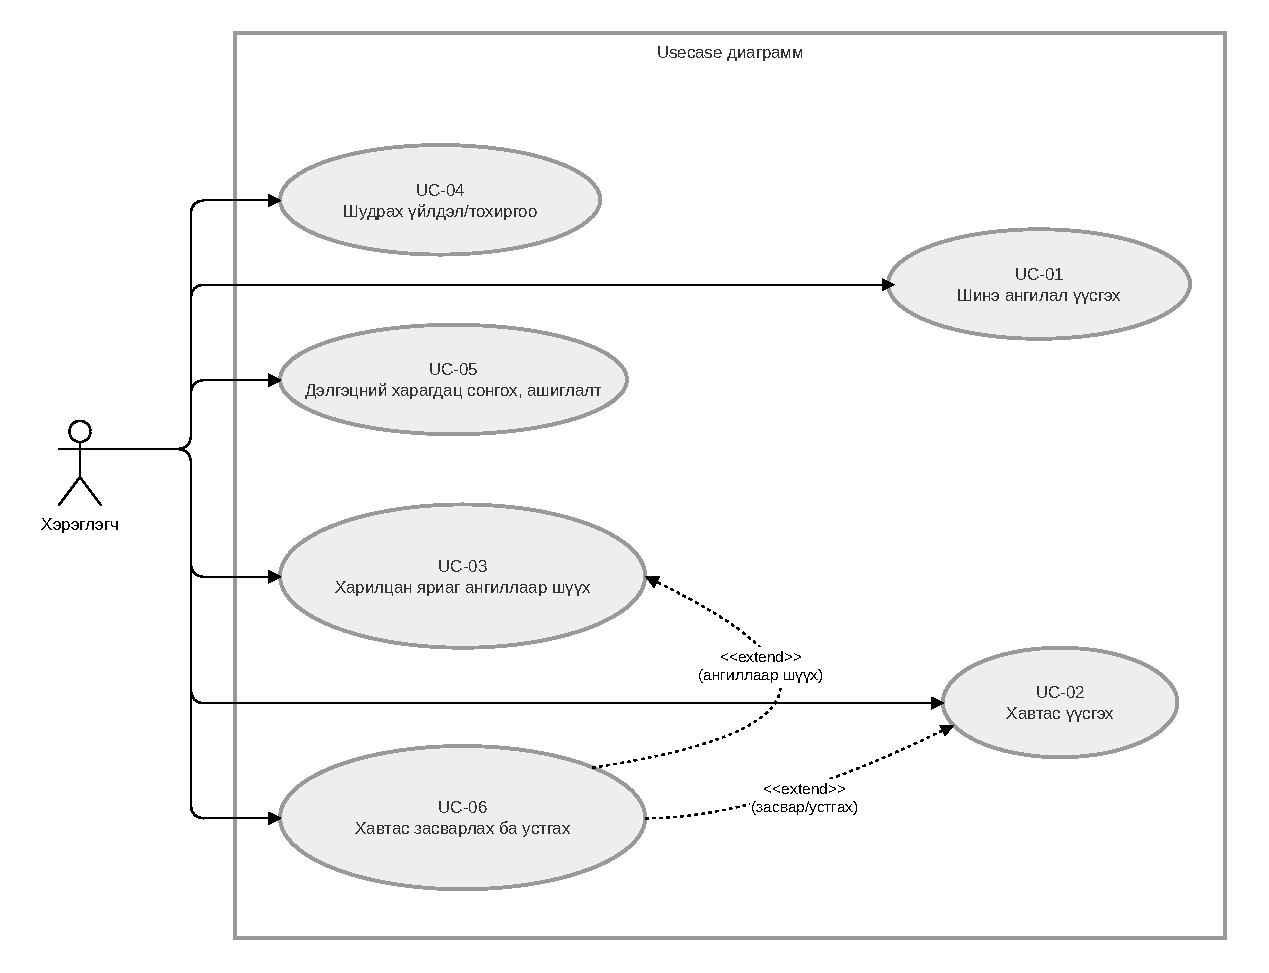
\includegraphics[width=0.85\textwidth]{Diagrams/usecase_diagram}
    \caption{Системийн хэрэглээний тохиолдлын диаграмм}
    \label{fig:usecase_diag}
\end{figure}

Дээрх диаграммд тусгагдсан үндсэн үйлдлүүдийн ажлын урсгал болон нөхцөлүүдийг дараах хүснэгтүүдээр дэлгэрэнгүй тайлбарлав.

% Хэрэглээний тохиолдол 1: Шошго үүсгэх
\begin{longtable}{|l|p{10.5cm}|}
    \caption{Хэрэглээний тохиолдол 1: Шошго үүсгэх} \label{tab:uc_create_category} \\
    \hline
    \textbf{ID / Нэр} & UC-01 / Шинэ шошго үүсгэх \\ \hline
    \textbf{Товч тайлбар} & Хэрэглэгч зурвас шүүх шинэ дүрэм (шошго) үүсгэж, нэр, өнгө болон шүүлтүүрүүдийг тохируулна. \\ \hline
    \textbf{Үйлдэгч} & Хэрэглэгч \\ \hline
    \textbf{Өмнөх нөхцөл} & Хэрэглэгч ``Шошго удирдах'' дэлгэцийг нээсэн байна. \\ \hline
    \textbf{Ажлын урсгал} &
    1. Хэрэглэгч ``+'' товчийг дарж үүсгэх цонхыг нээнэ. \newline
    2. Шошгоны нэрийг оруулж, жагсаалтаас өнгө сонгоно. \newline
    3. Шүүлтүүрийн төрлийг сонгоно: \newline
    \hspace{0.5cm} 3.1. Энгийн үг оруулах бол ``Энгийн үг нэмэх'' талбарт бичнэ. \newline
    \hspace{0.5cm} 3.2. Тогтмол илэрхийлэл (Regex) ашиглах бол дүрс дээр дарж паттерн оруулна. \newline
    4. Оруулсан өгөгдлийг шалгаж ``OK'' товчийг дарна. \\ \hline
    \textbf{Альтернатив} & Хэрэглэгч ``Cancel'' дарвал өөрчлөлт хадгалагдахгүй. Буруу тогтмол илэрхийллийн паттерн оруулбал систем алдаа заана. \\ \hline
    \textbf{Дараах нөхцөл} & Шинэ шошго баазад хадгалагдаж, зурвасууд шууд ангилагдана. \\ \hline
\end{longtable}

\vspace{1em}

% Хэрэглээний тохиолдол 2: Хавтас үүсгэх
\begin{longtable}{|l|p{10.5cm}|}
    \caption{Хэрэглээний тохиолдол 2: Хадгалсан харагдац (Хавтас) үүсгэх} \label{tab:uc_create_folder} \\
    \hline
    \textbf{ID / Нэр} & UC-02 / Хавтас үүсгэх \\ \hline
    \textbf{Товч тайлбар} & Хэрэглэгч өөрийн хэрэгцээнд тохирсон зурвасын харагдац (Хавтас) үүсгэж, доод навигацийн цэсэнд нэмнэ. \\ \hline
    \textbf{Үйлдэгч} & Хэрэглэгч \\ \hline
    \textbf{Ажлын урсгал} &
    1. Баруун дээд цэснээс ``Хавтас'' -> ``Харагдац үүсгэх'' сонгоно. \newline
    2. Хавтасны нэрийг бичиж, харагдах байрлал (index) болон өнгийг тодорхойлно. \newline
    3. ``OK'' товчийг дарж баталгаажуулна. \\ \hline
    \textbf{Дараах нөхцөл} & Шинэ хавтас доод навигацийн цэсэнд нэмэгдэж, хэрэглэгч тухайн хавтас руу автоматаар шилжинэ. \\ \hline
\end{longtable}

\vspace{1em}

% Хэрэглээний тохиолдол 3: Шошгоор шүүх
\begin{longtable}{|l|p{10.5cm}|}
    \caption{Хэрэглээний тохиолдол 3: Шошгоор шүүх} \label{tab:uc_filter_category} \\
    \hline
    \textbf{ID / Нэр} & UC-03 / Харилцан яриаг шошгоор шүүх \\ \hline
    \textbf{Товч тайлбар} & Хэрэглэгч үүсгэсэн хавтас доторх харилцан яриануудыг нэг болон хэд хэдэн шошгоор (Tag) шүүж харна. \\ \hline
    \textbf{Ажлын урсгал} &
    1. Хайх талбарын хажууд байрлах шүүлтүүрийн товчийг дарна. \newline
    2. Гарч ирэх жагсаалтаас нэг болон түүнээс дээш шошгыг сонгоно. \newline
    3. ``OK'' товчийг дарахад систем сонгосон шошгонд таарсан зурвасуудыг харуулна. \\ \hline
    \textbf{Дараах нөхцөл} & Жагсаалт шинэчлэгдэж, шүүлтийн төлөв хадгалагдана. \\ \hline
\end{longtable}

\vspace{1em}

% Хэрэглээний тохиолдол 4: Шудрах үйлдэл
\begin{longtable}{|l|p{10.5cm}|}
    \caption{Хэрэглээний тохиолдол 4: Шудрах үйлдлийн тохиргоо} \label{tab:uc_swipe_actions} \\
    \hline
    \textbf{ID / Нэр} & UC-04 / Шудрах үйлдлийн тохиргоо \\ \hline
    \textbf{Товч тайлбар} & Харилцан ярианы жагсаалтад зүүн эсвэл баруун тийш шудрахад хийгдэх үйлдлийг хэрэглэгч өөрөө сонгоно. \\ \hline
    \textbf{Ажлын урсгал} &
    1. Програмын ерөнхий тохиргооноос ``Шудрах үйлдэл'' хэсгийг нээнэ. \newline
    2. ``Эхнээс нь шудрах'' эсвэл ``Төгсгөлөөс нь шудрах'' сонголтыг дарна. \newline
    3. Боломжит үйлдлүүдээс (Устгах, Архивлах, Уншсан болгох г.м) нэгийг сонгоно. \\ \hline
    \textbf{Дараах нөхцөл} & Сонгосон үйлдэл тэр даруй хадгалагдаж, жагсаалт дээр ажиллаж эхэлнэ. \\ \hline
\end{longtable}

\vspace{1em}

% Хэрэглээний тохиолдол 5: Дэлгэцийн горим
\begin{longtable}{|l|p{10.5cm}|}
    \caption{Хэрэглээний тохиолдол 5: Дэлгэцийн харагдацын горим} \label{tab:uc_screen_view} \\
    \hline
    \textbf{ID / Нэр} & UC-05 / Screen View Mode сонгох \\ \hline
    \textbf{Товч тайлбар} & Нугалдаг төхөөрөмж эсвэл таблет дээр жагсаалт болон дэлгэрэнгүй хэсгийг хэрхэн харуулахыг тохируулна. \\ \hline
    \textbf{Ажлын урсгал} &
    1. Тохиргоо цэсний ``View mode'' хэсэгт орно. \newline
    2. ``Auto'', ``Single'', эсвэл ``Separated'' горимуудаас нэгийг сонгоно. \newline
    3. ``Auto'' горимд систем дэлгэцийн төлөвийг (Дэлгэц хаалттай/нээлттэй) мэдэрч автоматаар шилжинэ. \\ \hline
    \textbf{Дараах нөхцөл} & Програмын үндсэн дэлгэцийн бүтэц (layout) сонгосон горимын дагуу шинэчлэгдэнэ. \\ \hline
\end{longtable}

\vspace{1em}

% Хэрэглээний тохиолдол 6: Хавтас засварлах
\begin{longtable}{|l|p{10.5cm}|}
    \caption{Хэрэглээний тохиолдол 6: Хавтас засварлах ба устгах} \label{tab:uc_edit_folder} \\
    \hline
    \textbf{ID / Нэр} & UC-06 / Хавтас засах эсвэл устгах \\ \hline
    \textbf{Товч тайлбар} & Өмнө үүсгэсэн хавтасны мэдээллийг шинэчлэх эсвэл системээс бүрмөсөн устгана. \\ \hline
    \textbf{Ажлын урсгал} &
    1. Доод навигацийн цэс дээрх хавтасны дүрс дээр удаан дарна. \newline
    2. Мэдээллийг (нэр, өнгө, байрлал) засаад ``OK'' дарах эсвэл ``Delete'' товчийг сонгоно. \newline
    3. Устгах үйлдэл дээр систем дахин баталгаажуулалт асууна. \\ \hline
    \textbf{Дараах нөхцөл} & Өөрчлөлт хадгалагдах эсвэл хавтас навигацийн цэснээс алга болж хэрэглэгч үндсэн харагдац руу шилжинэ. \\ \hline
\end{longtable}


% ============================================================
% Section 3: Системийн архитектур
% ============================================================
\section{Системийн архитектур}
Системийн ерөнхий архитектурыг Зураг \ref{fig:architecture} уламжлалт 3 давхаргат (3-Layer Architecture) бүтцээр зохиомжилсон бөгөөд энэ нь өгөгдлийн, логик болон хэрэглэгчийн харилцах цонхны хэсгүүдийг бие даан хөгжүүлэх, турших боломжийг олгосон.

\begin{itemize}
    \item \textbf{Өгөгдлийн давхарга (Data Layer)}: Room Persistence Library ашиглан локал SQLite баазад зурвас, харилцан яриа болон ангиллын мэдээллийг хадгална.
    \item \textbf{Бизнес логикийн давхарга (Domain Layer)}: Тогтмол илэрхийллийн шүүлтүүрийн хөдөлгүүр болон хавтаслах системийн цөм логик байрлана.
    \item \textbf{Танилцуулга давхарга (Presentation Layer)}: XML View систем болон Jetpack Compose ашиглан хэрэглэгчийн харилцах цонхыг бүрдүүлнэ.
\end{itemize}

\begin{figure}[H]
    \centering
    
\includegraphics[width=0.55\textwidth]{Diagrams/architecture}
    \caption{Системийн ерөнхий бүтэц (Architecture Diagram)}
    \label{fig:architecture}
\end{figure}

% ============================================================
% Section 4: Өгөгдлийн сангийн зохиомж
% ============================================================
\section{Өгөгдлийн сангийн зохиомж}
Өгөгдлийн сангийн гол бүтэц, хүснэгт хоорондын холбоосыг ER диаграммаар Зураг~\ref{fig:erd} дээр үзүүлэв.

\begin{figure}[H]
    \centering
    
\includegraphics[width=0.55\textwidth]{Diagrams/erd}
    \caption{Өгөгдлийн сангийн ерөнхий бүтэц (ER Diagram)}
    \label{fig:erd}
\end{figure}

\begin{itemize}
    \item \textbf{Categories}: Ангиллын нэр, өнгө, дүрмийн тохиргоо хадгална.
    \item \textbf{Rules}: Түлхүүр үг болон тогтмол илэрхийллийн дүрэм, ангилалтай холбогдоно.
    \item \textbf{Харилцан яриа}: Харилцан ярианы ерөнхий мэдээлэл, ангиллын холбоос.
    \item \textbf{Messages}: Бодит зурвасын агуулга, илгээгч, огноо, харилцан ярианд хамаарал.
\end{itemize}

\subsection{Өгөгдлийн сангийн шинэчлэл}
Төслийн хүрээнд \texttt{MessagesDatabase}-ийн хувилбарыг 10-аас 13 болгон ахиулж, дараах өөрчлөлтүүдийг хийсэн:
\begin{itemize}
    \item \textbf{MIGRATION 10--11}: \texttt{categories} хүснэгтийг шинээр үүсгэж, \texttt{messages} болон \texttt{conversations} хүснэгтүүдэд ангиллын мэдээллийг хадгалах (\texttt{category}, \texttt{categoryId}) талбаруудыг нэмсэн.
    \item \textbf{MIGRATION 11-12}: Түлхүүр үг нь тогтмол илэрхийлэл (Regex) эсэхийг тодорхойлох \texttt{keywords\_is\_regex} баганыг нэмж, шүүлтийн логикийг өргөтгөсөн.
    \item \textbf{MIGRATION 12--13}: Шүүлтүүрийн логикийг илүү нарийвчлалтай болгох зорилгоор \texttt{categories} хүснэгтэд \texttt{plain\_keywords} болон \texttt{regex\_patterns} багануудыг шинээр нэмж, "Dual-mode" шүүлтийг зэрэг ажиллуулах нөхцөлийг бүрдүүлсэн.
\end{itemize}

\begin{figure}[H]
    \centering
    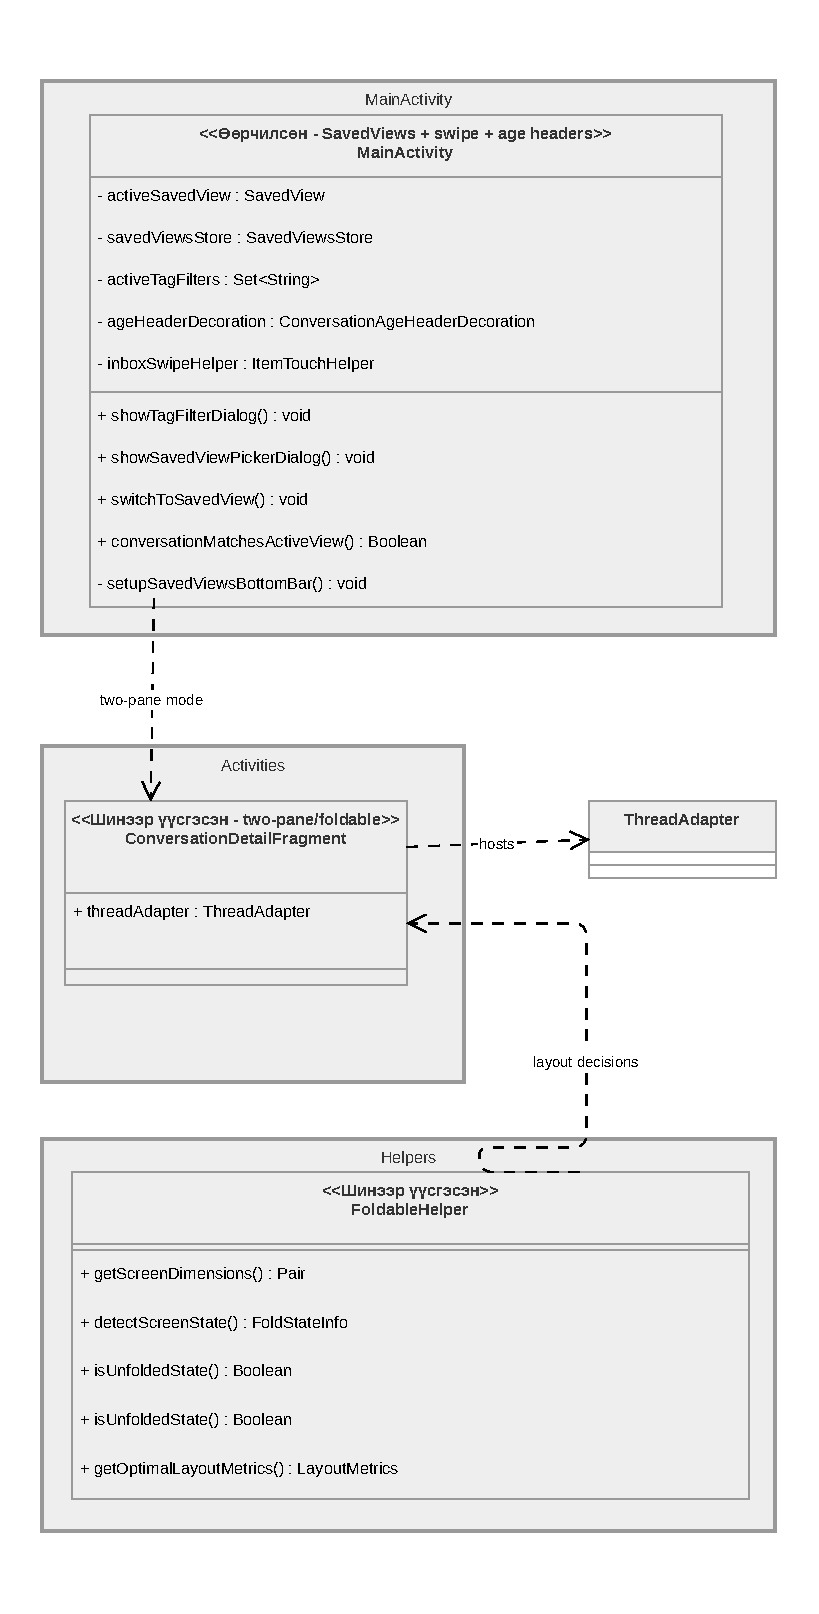
\includegraphics[width=0.9\textwidth]{Diagrams/class/database}
    \caption{Өгөгдлийн сангийн бүтэц болон DAO-ийн класс диаграмм}
    \label{fig:db_schema}
\end{figure}

% ============================================================
% Section 5: Нарийвчилсан зохиомж ба логик дараалал
% ============================================================
\section{Нарийвчилсан зохиомж ба Логик дараалал}
Системийн хамгийн чухал процесс болох ``Ангилал үүсгэх, түүний хэрэгжилт''-ийн логикийг UML Sequence диаграммаар (Зураг~\ref{fig:seq_diag}) харуулав. Диаграммд хэрэглэгчийн ангиллын нэр, өнгө болон түлхүүр үгсийг оруулах үйлдэл, өгөгдлийн сан руу хадгалах процесс, мөн тухайн ангиллын дагуу зурвасыг автоматаар ангилах үйл явцын урсгалыг харуулсан.

\begin{figure}[H]
    \centering
    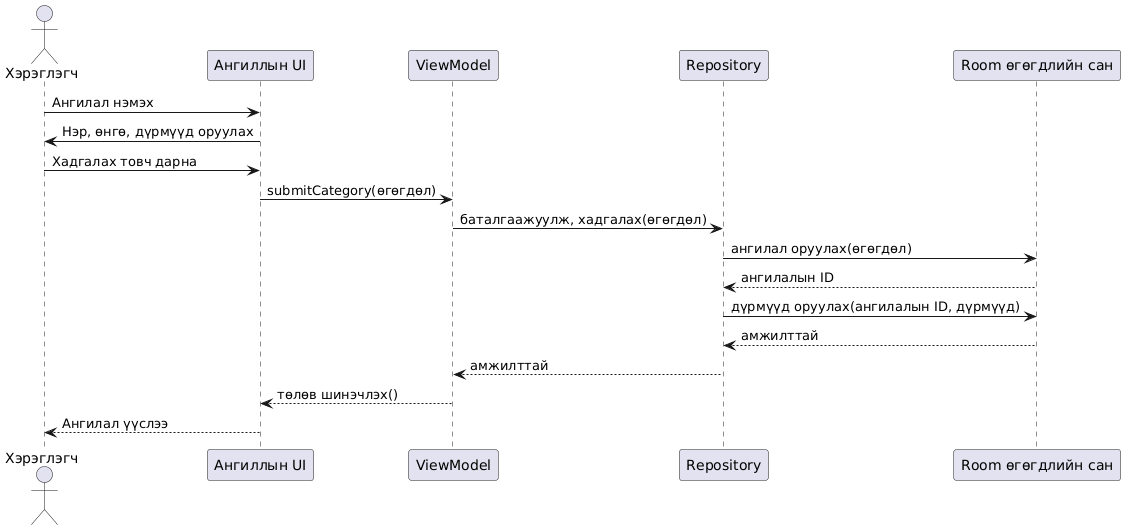
\includegraphics[width=0.85\textwidth]{Diagrams/sequence/category_sequence}
    \caption{Ангилал шинээр үүсгэх (Sequence Diagram)}
    \label{fig:seq_diag}
\end{figure}

Хавтас үүсгэх болон хадгалах логикийг дарааллын диаграммаар (Зураг~\ref{fig:seq_category}) харуулав. Хавтас үүсгэх, тохируулах үйлдэл төстэй бүтэцтэй бөгөөд өгөгдлийн нэгдсэн урсгал хэсэгт аль алинд ижилхэн процессуудыг агуулдаг тул нэг диаграммд цэнхэр өнгө бүхий хэсэгт нэгтгэн үзүүлэв. Улаан өнгөөр тэмдэглэсэн хэсэг нь ангиллын дүрмийн тохиргоонуудын нэг болох устгах үйлдлийг харуулсан.

\begin{figure}[H]
    \centering
    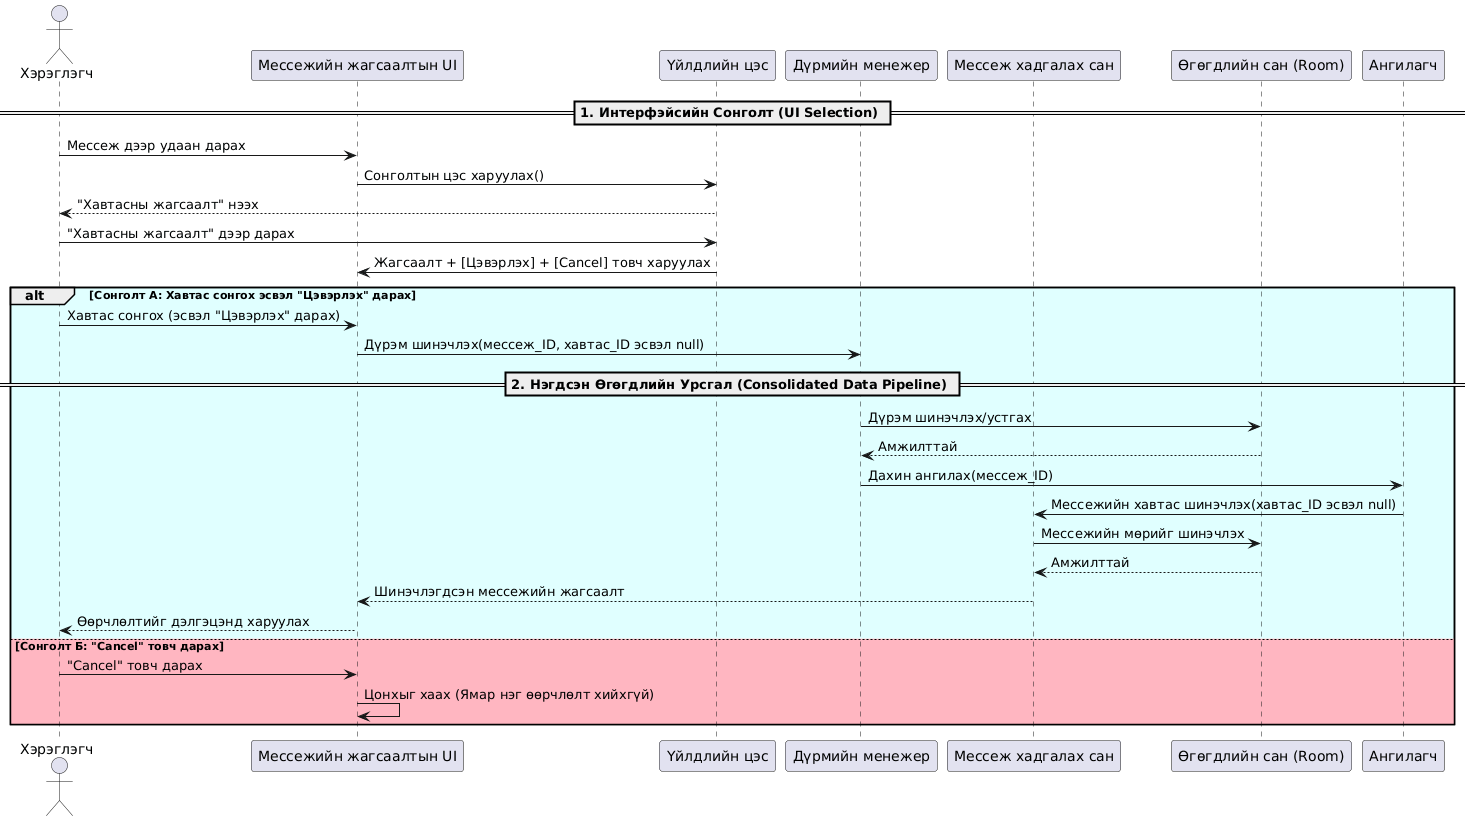
\includegraphics[width=0.85\textwidth]{Diagrams/sequence/assign_folder_sequence.png}
    \caption{Хавтас үүсгэх болон хадгалах дараалал (Sequence Diagram)}
    \label{fig:seq_category}
\end{figure}

Мөн харилцан яриан дээр удаан дарснаар гарч ирэх доод хэсгийн тохиргоо гарч ирж тэдгээрээс сонгох явцыг үйл ажиллагааны диаграммаар (Зураг~\ref{fig:act_diag}) дүрслэв. Хавтас оноохоос гадна бусад үндсэн үйлдлүүдийг (архивлах, устгах, уншсан төлөв солих) нэгтгэн харуулсан бөгөөд тэдгээр үйлдэлийг үр дүнг нарийн тайлбарлахгүйгээр үр дүнг төгсгөл хэсэг рүү шууд чиглүүлсэн.

\begin{figure}[H]
    \centering
    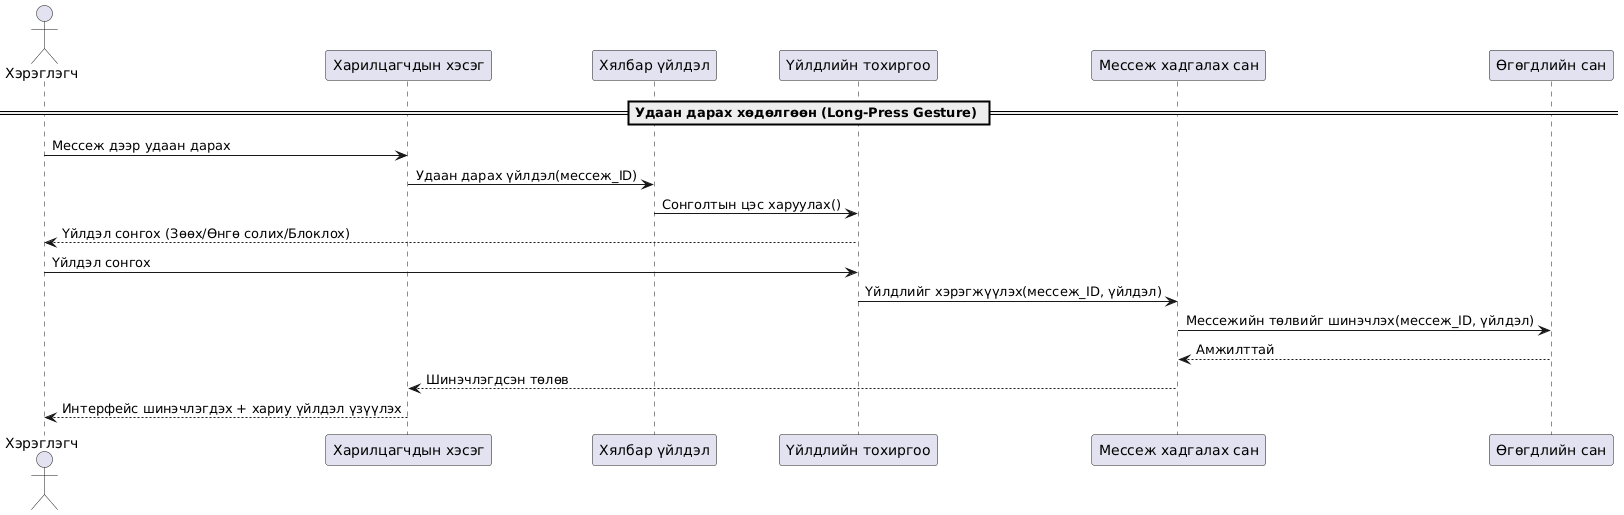
\includegraphics[width=0.85\textwidth]{Diagrams/sequence/long_press_sequence_diagram}
    \caption{Удаан дарж гарч ирэх туслах цэсний логик}
    \label{fig:act_diag}
\end{figure}

\section{Төслийн суурь бүтэц (Fossify Messages)}
Fossify Messages (мөн өмнөх Simple Mobile Tools) төслийн сангуудын бүтэц нь Android хөгжүүлэлтийн стандарт болон Separation of Concerns (үүрэг хариуцлагыг тусгаарлах) зарчмыг баримталдаг. Үндсэн хавтаснуудын үүргийг доор дэлгэрэнгүй тайлбарлав.

\begin{itemize}
    \item \textbf{activities/ (Presentation Layer)}: Энэ санд аппликейшны бүх дэлгэцүүд (UI screens) байрлана. Жишээ нь: \texttt{MainActivity} (мессежийн жагсаалт), \texttt{ThreadActivity} (тухайн харилцагчтай харилцсан түүх), \texttt{SettingsActivity}. Android-ийн ажиллах үндсэн цэгүүд энд байна.

    \item \textbf{adapters/ (UI Logic)}: Жагсаалттай ажилладаг классууд байрлана. \texttt{RecyclerView}-д өгөгдлийг (мессеж, харилцан яриа) хэрхэн харуулахыг зохицуулдаг. Жишээ нь: \texttt{ThreadAdapter} нь чат доторх мессеж бүрийн харагдах байдлыг удирддаг.

    \item \textbf{App.kt (Global Configuration)}: Аппликейшн ажиллахад хамгийн түрүүнд дуудагддаг класс. Энд глобал тохиргоонууд, Dependency Injection (DI)-ийн эхлэл, эсвэл өгөгдлийн сангийн бэлтгэл ажил хийгддэг.

    \item \textbf{databases/ (Data Layer)}: Room Persistence Library ашиглан локал өгөгдлийн сантай харьцах хэсэг. Энд \texttt{MessagesDatabase}, \texttt{ConversationsDao} зэрэг классууд байрлаж, SQLite-аас өгөгдөл унших, бичих үйлдлийг гүйцэтгэнэ.

    \item \textbf{dialogs/ (Reusable UI)}: Хэрэглэгчээс баталгаажуулалт авах, текст оруулах зэрэг жижиг цонхнууд (Pop-ups) энд байна. Жишээ нь: Мессеж устгах үеийн "Энэ үйлдлийг хийхдээ итгэлтэй байна уу?" цонх. Энэ нь элементийг дахин ашиглах \cite{design_patterns} зохистой арга юм.

    \item \textbf{extensions/ (Kotlin Power)}: Fossify төслүүдийн нэг онцлог бол Extension Functions маш их ашигладаг. Суурь классууд дээр (жишээ нь \texttt{Context}, \texttt{String}, \texttt{Long}) нэмэлт функц бичиж, кодыг эмх замбараагүй болохоос сэргийлдэг. Жишээ нь: \texttt{Long.formatDate()} гэх мэт.

    \item \textbf{helpers/ (Utilities)}: Туслах функцүүд болон тогтмол утгууд (Constants) байрлана. Мөн Prefs буюу хэрэглэгчийн тохиргоог (\texttt{SharedPrefs}) удирдах классууд энд байна.

    \item \textbf{interfaces/ (Abstraction)}: Классууд хоорондоо харилцах гүүр болох "Listener"-үүд байрлана. Жишээ нь: \texttt{RefreshMessagesListener} – өгөгдөл өөрчлөгдөхөд UI-г шинэчлэх үүрэгтэй.

    \item \textbf{messaging/ (Core Logic)}: Мессеж илгээх, хүлээн авах, SMS/MMS-ийн төрлийг тодорхойлох зэрэг системийн хамгийн чухал логикууд энд байрладаг. Энэ бол апп-ын "зүрх" нь юм.

    \item \textbf{models/ (Data Classes)}: Өгөгдлийн бүтэц буюу POJO классууд. Жишээ нь: \texttt{Message}, \texttt{Conversation}, \texttt{Contact} гэх мэт өгөгдлийн загварууд.

    \item \textbf{receivers/ (Android Components)}: Android системээс ирж буй дохиог (Broadcast) барьж авах хэсэг. Хамгийн чухал нь \texttt{SmsReceiver} буюу шинэ мессеж ирэхэд түүнийг барьж аваад апп-д мэдэгдэх үүрэгтэй.

    \item \textbf{services/ (Background Tasks)}: Ар талд (Background) ажиллах шаардлагатай ажлууд. Жишээ нь: Мессеж илгээх процесс дуустал ажиллах үйлчилгээ энд байна.

    \item \textbf{ui/ (Custom UI)}: Апп-д ашиглагдаж буй тусгайлан загварчилсан (Custom) View-үүд байрлана. Жишээ нь: Өнгө сонгогч, тусгай товчлуур гэх мэт.
\end{itemize}
% ============================================================
% Section 6: Класс диаграммууд
% ============================================================
\section{Системийн класс диаграммууд}

\subsection{Activity болон UI логикийн бүтэц}
Аппликейшны дэлгэцүүд болон тэдгээрийн хоорондын харилцан хамаарлыг Зураг~\ref{fig:class_activity}-д үзүүлэв.

\begin{figure}[H]
    \centering
    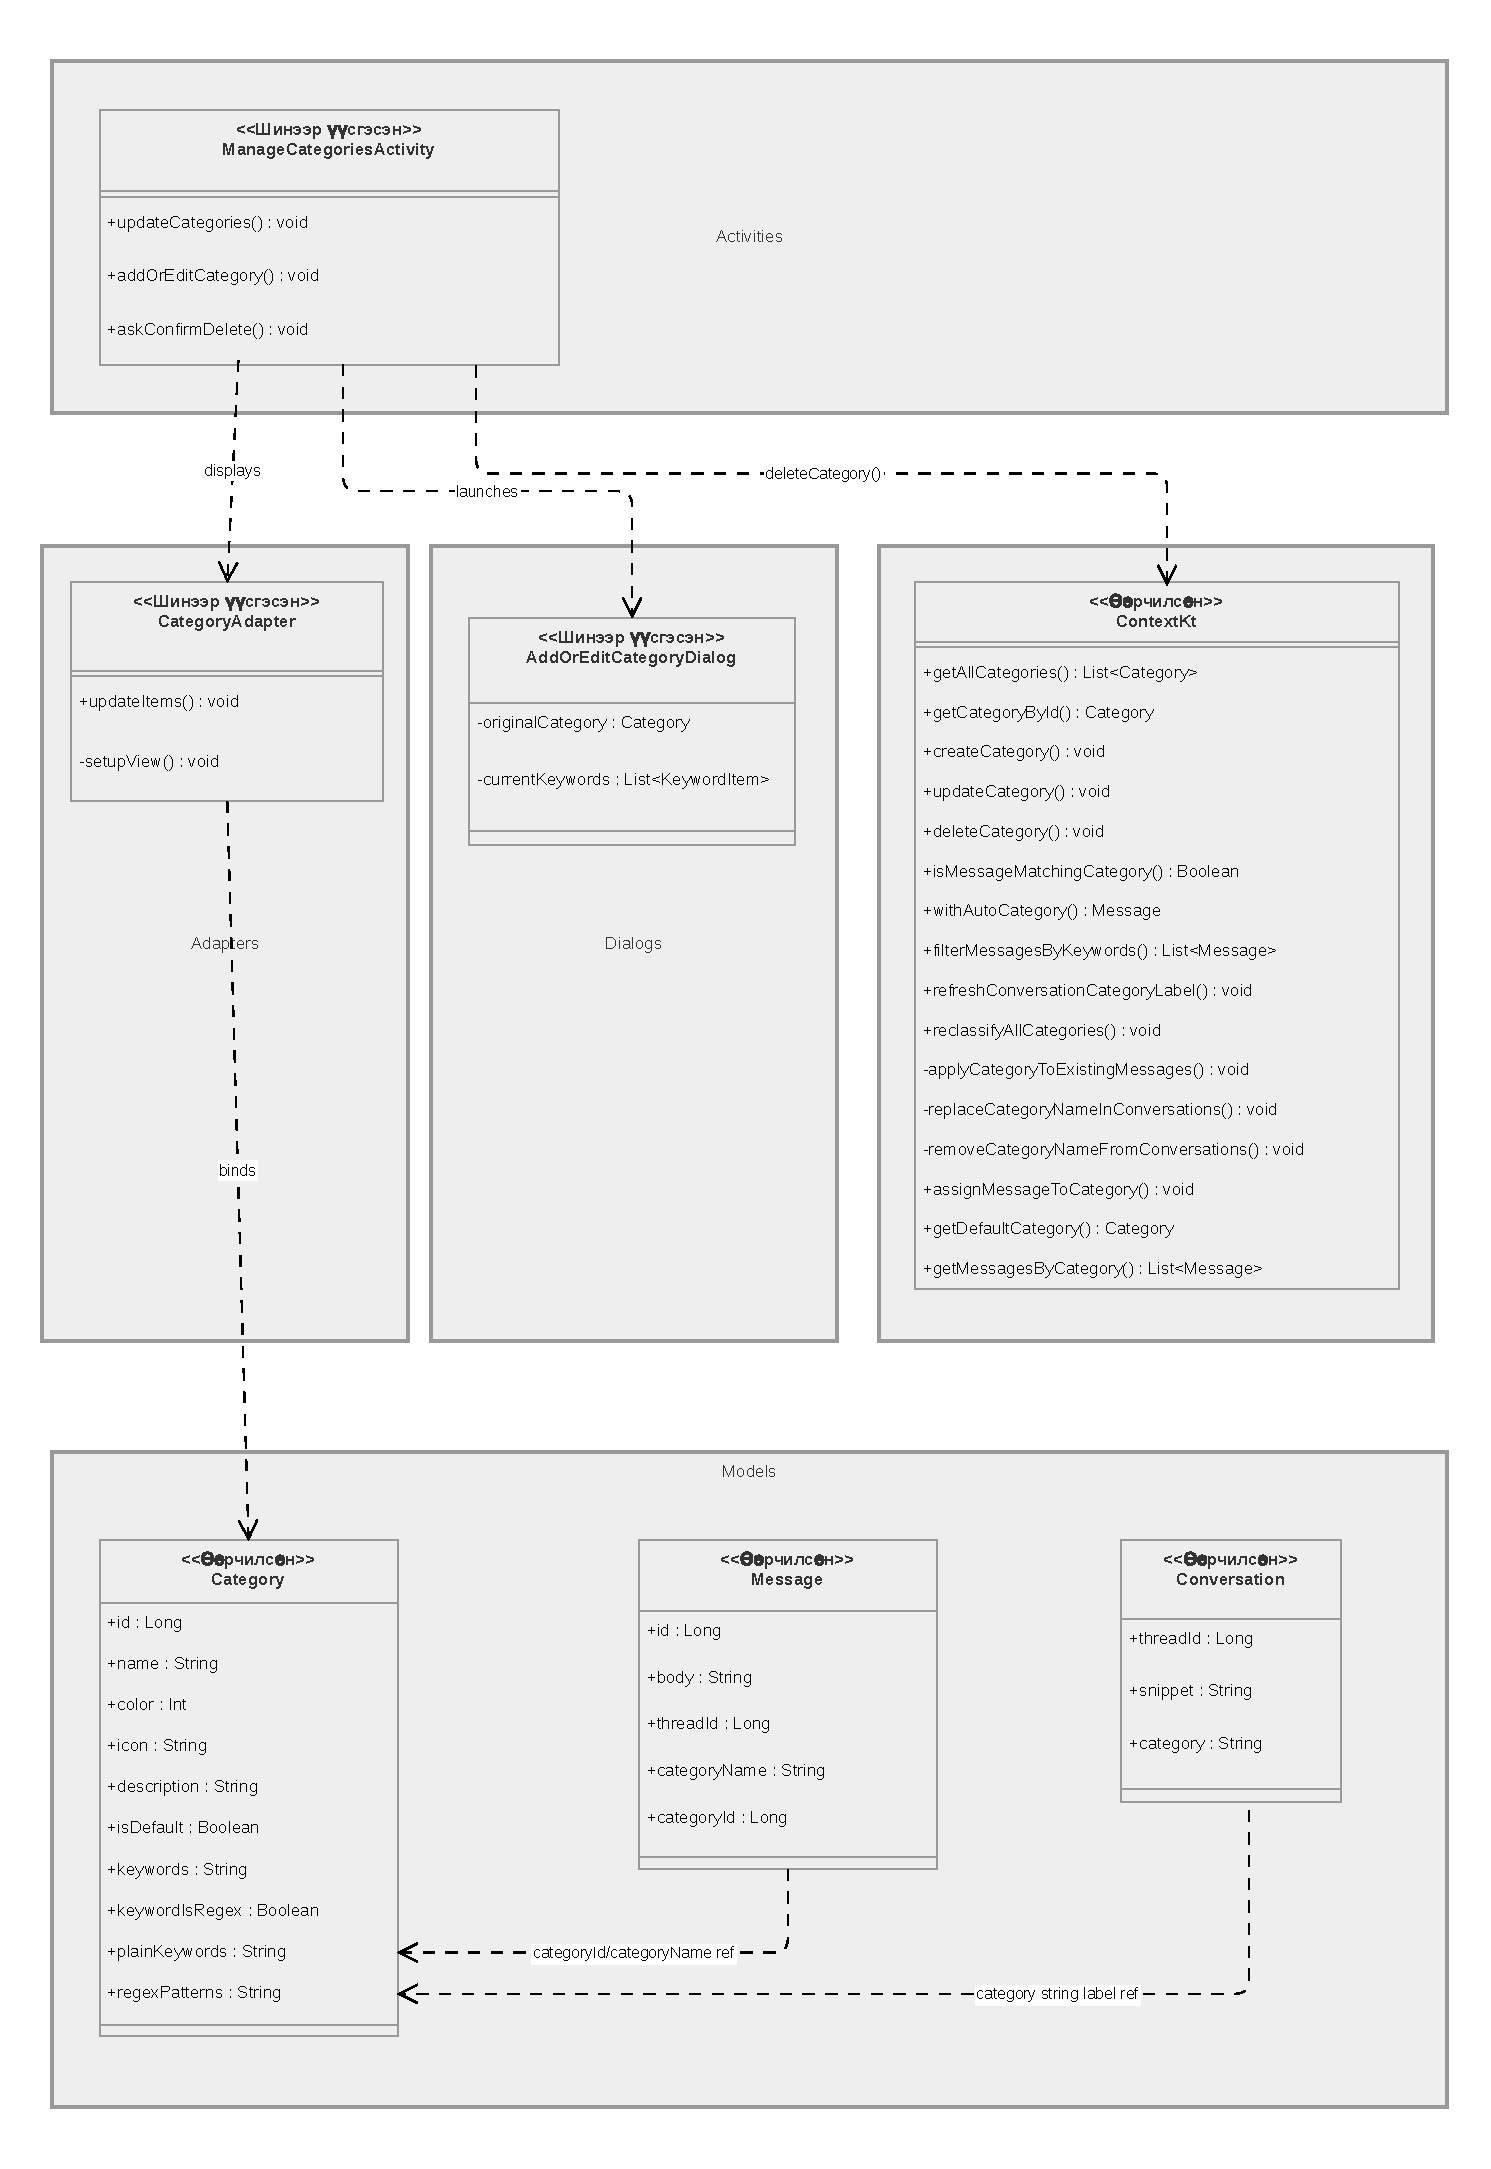
\includegraphics[width=0.85\textwidth]{Diagrams/class/activity}
    \caption{Үндсэн Activity, Fragment болон UI логикийн класс диаграмм}
    \label{fig:class_activity}
\end{figure}

\noindent \textbf{Гол классуудын үүрэг:}
\begin{itemize}
    \item \textbf{ManageCategoriesActivity}: Ангиллын жагсаалтыг шинэчлэх (\texttt{updateCategories}), засах цонх дуудах (\texttt{addOrEditCategory}) үйлдлүүдийг удирдана.
    \item \textbf{MainActivity}: Хадгалсан харагдацуудыг (SavedViewsStore), хугацааны бүлэглэлт (AgeHeaderDecoration), шудрах үйлдэл (inboxSwipeHelper) зэрэг шинэ боломжуудыг нэгтгэсэн.
    \item \textbf{ContextKt}: Системийн бизнес логикийн гол цөм бөгөөд \texttt{withAutoCategory()}, \texttt{refreshConversationCategoryLabel()}, \texttt{filterMessagesByKeywords()} зэрэг өргөтгөл функцүүдийг агуулна.
\end{itemize}

\subsection{Ангилал болон шүүлтүүрийн системийн бүтэц}
Зурвас таних, ангилал үүсгэх болон өгөгдлийн сангийн харилцан хамаарлыг Зураг~\ref{fig:class_category}-д үзүүлэв.

\begin{figure}[H]
    \centering
    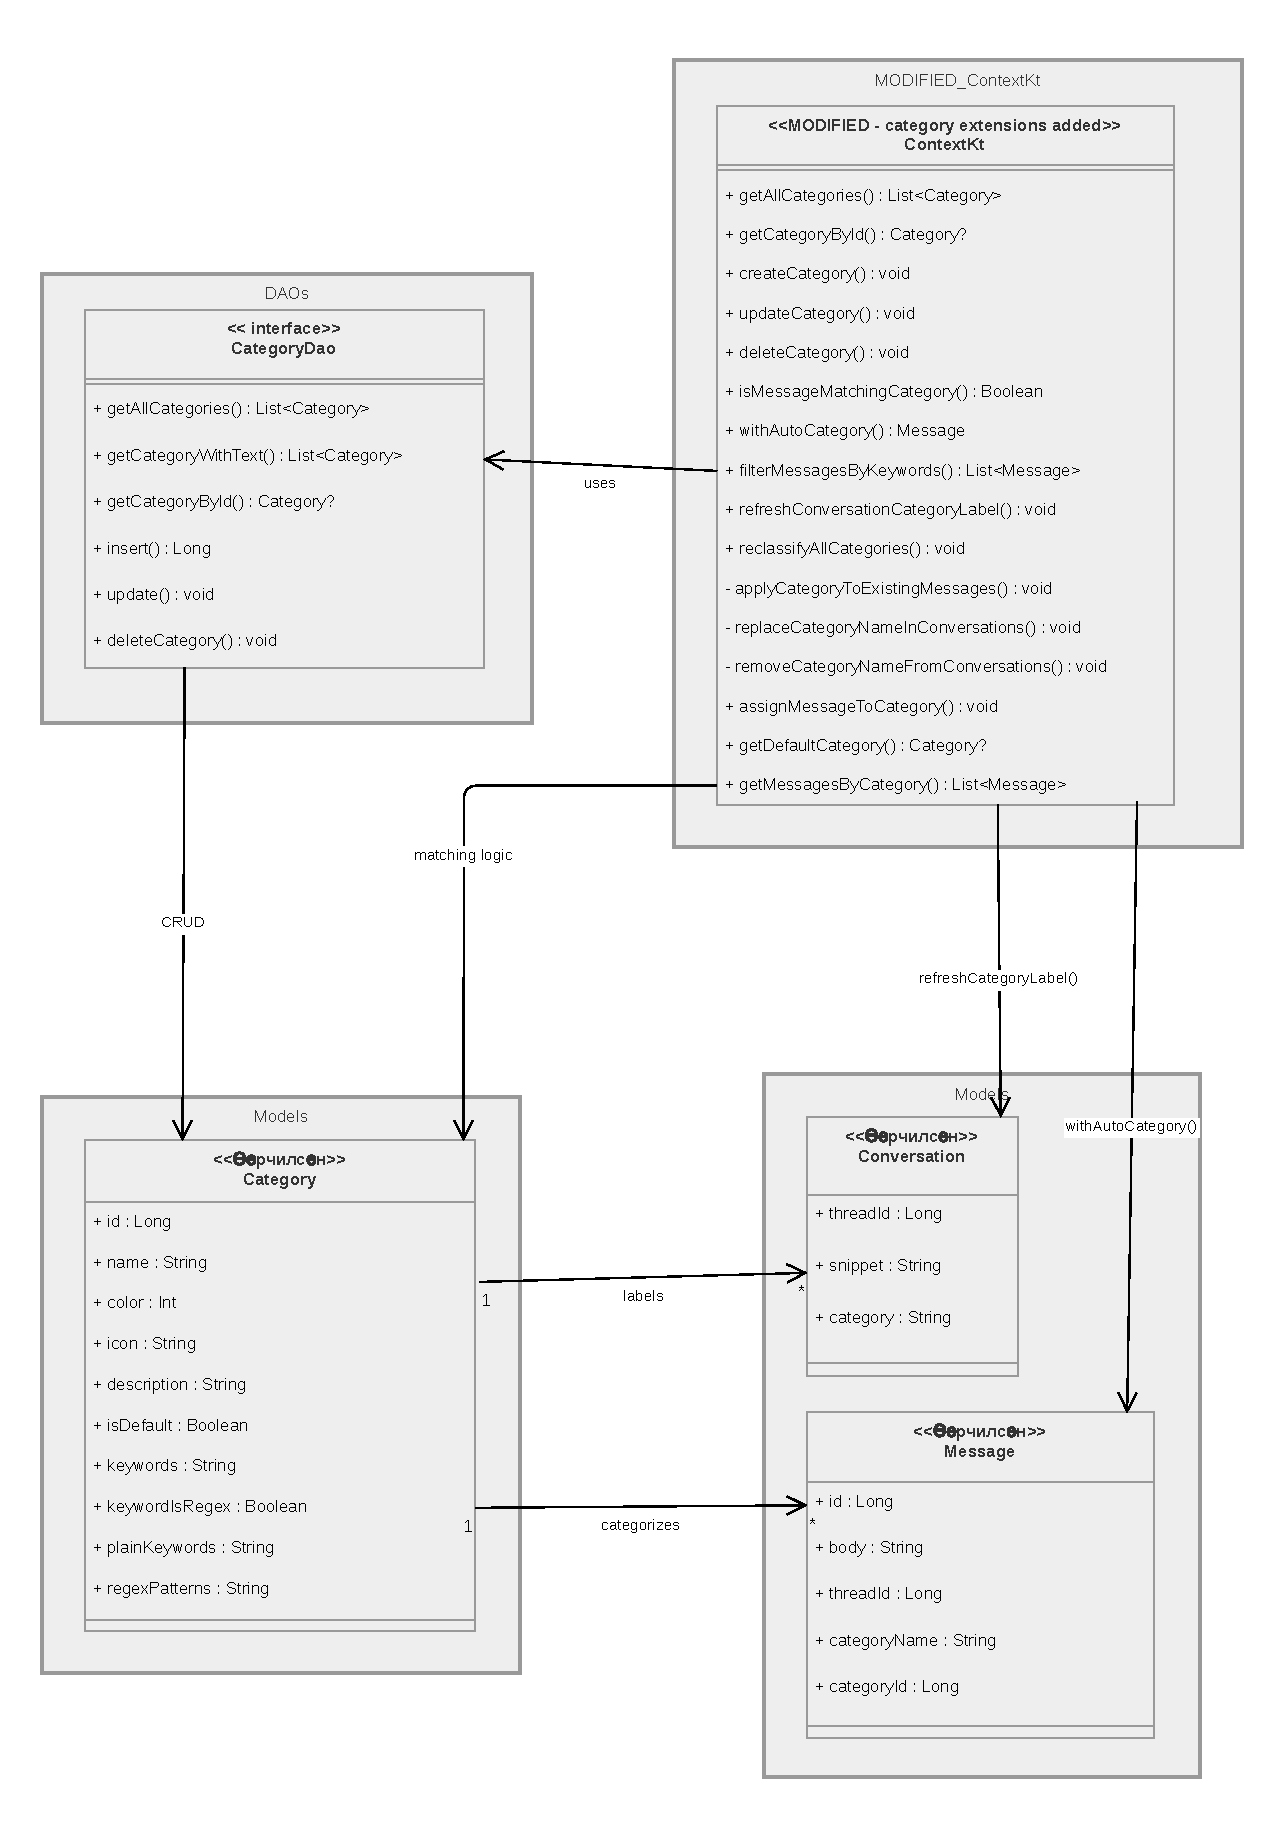
\includegraphics[width=0.85\textwidth]{Diagrams/class/category}
    \caption{Ангилал болон шүүлтүүрийн нарийвчилсан класс диаграмм}
    \label{fig:class_category}
\end{figure}

\noindent \textbf{Бүрэлдэхүүн хэсгүүдийн тайлбар:}
\begin{itemize}
    \item \textbf{CategoryDao}: Ангиллын жагсаалт авах (\texttt{getAllCategories}), түлхүүр үгээр хайх (\texttt{getCategoryWithText}) болон CRUD үйлдлүүдийг гүйцэтгэнэ.
    \item \textbf{Category загвар}: \texttt{plainKeywords} болон \texttt{regexPatterns} талбаруудыг ашиглан ``Dual-mode'' шүүлтүүрийг дэмжинэ.
    \item \textbf{Message загвар}: \texttt{categoryId} болон \texttt{categoryName} талбараар дамжуулан \texttt{Category} загвартай холбогдоно.
\end{itemize}

\subsection{Түлхүүр үгсийн удирдлагын систем ба Compose зохиомж}
Ангиллын дүрмүүдийг удирдах хэрэглэгчийн харилцах цонхны бүтцийг Зураг~\ref{fig:class_ui}-д үзүүлэв.

\begin{figure}[H]
    \centering
    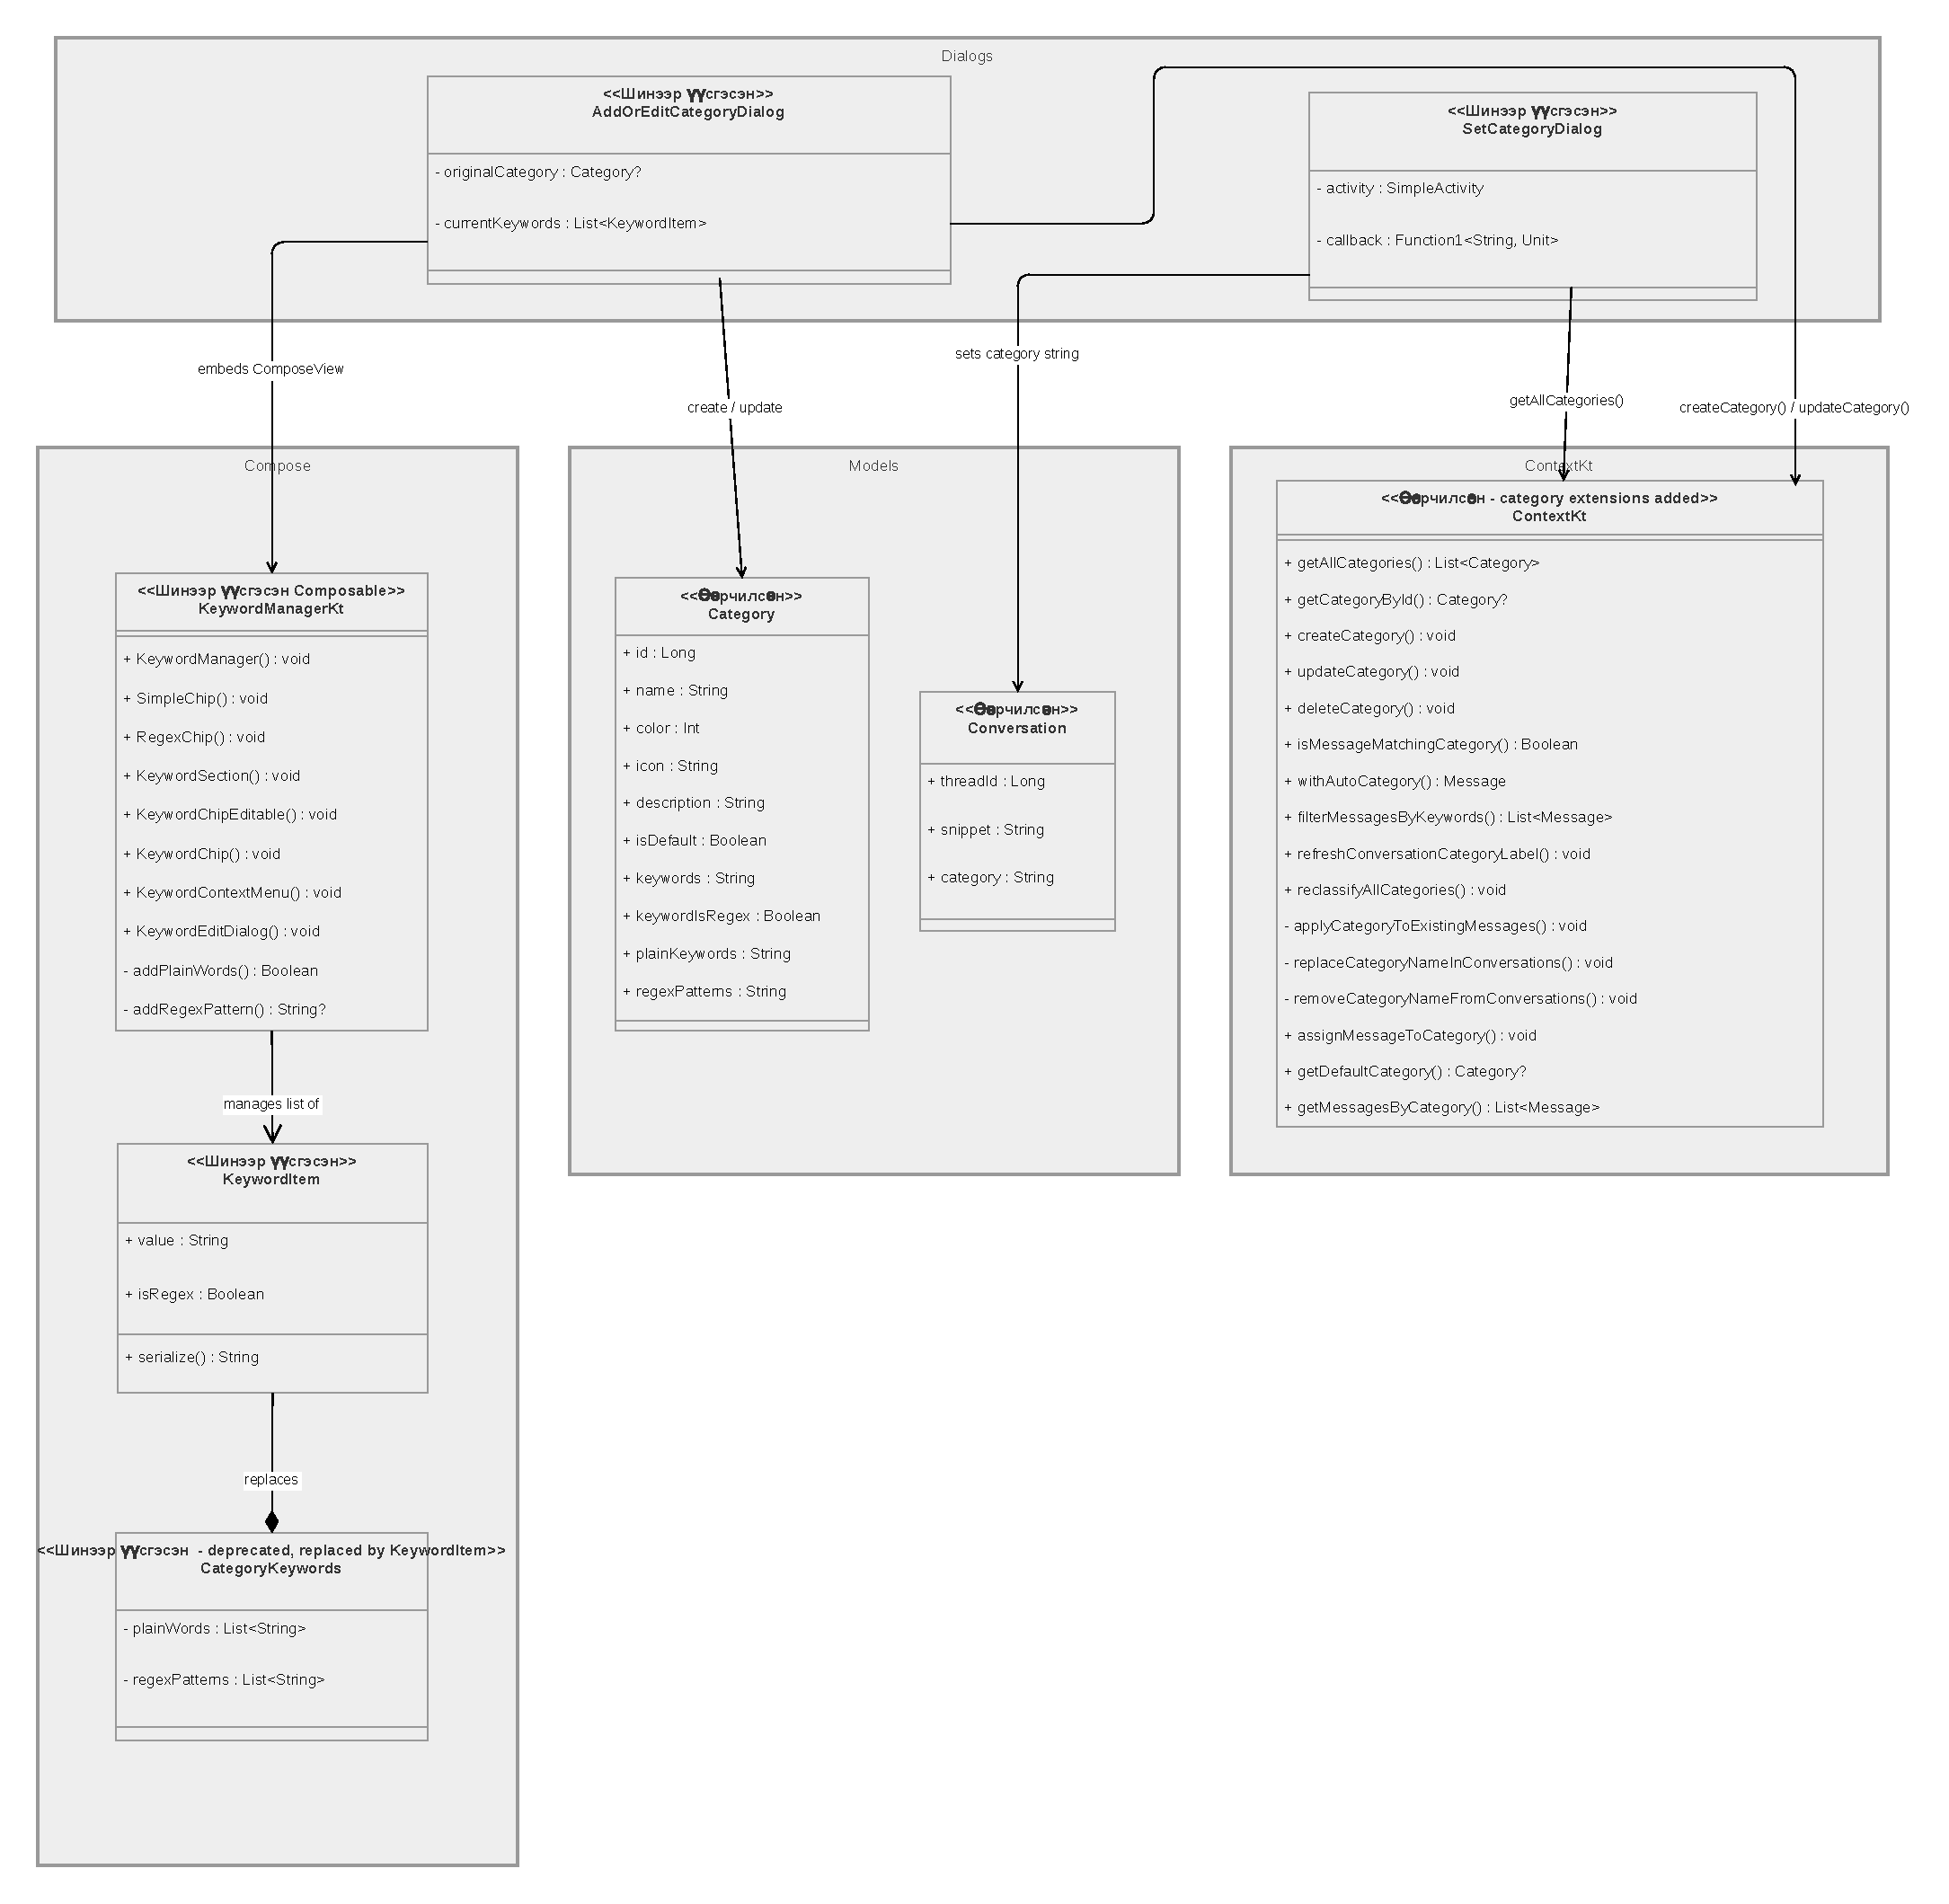
\includegraphics[width=0.85\textwidth]{Diagrams/class/keyboard_ui}
    \caption{Түлхүүр үг удирдах хэрэглэгчийн харилцах цонх болон Compose компонентуудын класс диаграмм}
    \label{fig:class_ui}
\end{figure}

\begin{itemize}
    \item \textbf{KeywordManagerKt}: Түлхүүр үгсийн удирдлагын үндсэн Composable класс. Чип хэлбэртэй харагдацууд (\texttt{SimpleChip}, \texttt{RegexChip}), засах цонх болон контекст цэсийг агуулна.
    \item \textbf{AddOrEditCategoryDialog}: Уламжлалт View систем болон Compose-ийг нэгтгэсэн гүүр. \texttt{createCategory()} болон \texttt{updateCategory()} функцүүдийг дуудаж өгөгдлийг хадгална.
\end{itemize}

% ============================================================
% Section 7: UI/UX зохиомж
% ============================================================
\section{Хэрэглэгчийн харилцах цонхны зохиомж}
Хэрэглэгчийн харилцах цонхыг Material Design 3 стандартын~\cite{material_design} дагуу зохиомжилсон.
\begin{itemize}
    \item \textbf{Adaptive Layout}: Нугалдаг төхөөрөмж нээгдэх үед WindowInfoTracker ашиглан дэлгэцийн талбайг мэдэрч, хоёр баганат харагдац руу автоматаар шилжинэ.
    \item \textbf{Хадгалсан харагдац}: Хавтас тус бүрт өөрийн гэсэн өнгө оноож, харилцан ярианы жагсаалтыг тухайн өнгөөр харуулна.
    \item \textbf{Keyword Manager}: Тогтмол илэрхийлэл болон түлхүүр үгсийг нэг дороос удирдах боломжтой интерактив цонхыг Jetpack Compose-оор хэрэгжүүлсэн.
\end{itemize}

Доод цэсийг эрхий хурууны идэвхтэй бүсэд байрлуулах нь нэг гараар ашиглах эргономикийг сайжруулж \cite{hurff2016thumb}, шудрах үйлдлүүдээр архивлах, уншсан төлөв солих, хавтас оноох зэрэг үйлдлийг нэг алхамд гүйцэтгэх боломж бүрдүүлсэн.

% ============================================================
% Section 8: Аюулгүй байдлын зохиомж
% ============================================================
\section{Аюулгүй байдлын зохиомж}
Хэрэглэгчийн хувийн зурвасын нууцлалыг хангах үүднээс дараах арга хэмжээнүүдийг зохиомжид тусгав:
\begin{itemize}
    \item \textbf{On-device Filtering}: Зурвасыг ангилах бүх процесс зөвхөн төхөөрөмж дээр локал байдлаар хийгдэх бөгөөд гадны сервер рүү өгөгдөл дамжуулахгүй.
    \item \textbf{Local-first Database}: Өгөгдлийн сан нь Android-ийн App Sandbox \cite{android_app_sandbox} дотор тусгаарлагдсан тул бусад аппликейшн шууд хандах боломжгүй.
\end{itemize}
 % Арга зүй ба системийн зохиомж
    \chapter{Шаардлага ба төлөвлөлт}

\section{Функционал шаардлага (Functional Requirements)}
Системийн гүйцэтгэх үндсэн үйлдлүүдийг SRS стандартын дагуу \cite{ieee1998srs} дараах байдлаар тодорхойлов.
\begin{enumerate}[label=FR\arabic*.]
    \item \textbf{Тогтмол илэрхийлэлд суурилсан танилт}: Хэрэглэгчийн тохируулсан тогтмол илэрхийлэл ашиглан ирж буй зурвасыг автоматаар таньж, ангилах.
    \item \textbf{Харилцан ярианы ангиллын шошголол}: Харилцан яриа бүрт тухайн зурваст тохирох өнгөт шошго оноож, харагдах байдлыг ялгах.
    \item \textbf{Дасан зохицох хэрэглэгчийн харилцах цонхны дэмжлэг}: Нугалдаг төхөөрөмж нээгдэх үед хэрэглэгчийн харилцах цонхыг хоёр баганат харагдац руу гацалтгүйгээр шилжүүлэх.
    \item \textbf{Шудрах үйлдлийн тохиргоо}: Харилцан яриаг баруун, зүүн тийш шудрах үйлдлээр устгах, архивлах зэрэг үйлдлийг хурдан гүйцэтгэх.
    \item \textbf{Хугацааны бүлэглэлт}: Inbox дахь зурвасуудыг Өнөөдөр'', Өчигдөр'', Энэ сар'' гэсэн гарчиг дор автоматаар бүлэглэх.
\end{enumerate}

\section{Функционал бус шаардлага (Non-Functional Requirements)}
Системийн чанар болон найдвартай ажиллагааг хангах дараах шаардлагуудыг тавьсан:
\begin{itemize}
    \item \textbf{Гүйцэтгэл}: 1,000-аас дээш харилцан яриатай үед жагсаалт секундэд 60 frame хурдтай (smooth scroll) ажиллах.
    \item \textbf{Аюулгүй байдал}: Зурвасын агуулгыг гадагш дамжуулахгүй, бүх шүүлтүүрийг локал төхөөрөмж дээр (On-device) ажиллуулах.
    \item \textbf{Найдвартай байдал}: Room өгөгдлийн сангийн \cite{room_guide} шилжилт хийх үед хэрэглэгчийн өмнөх өгөгдөл алдагдахгүй байх.
    \item \textbf{Уян хатан байдал}: Шүүлтүүрийн дүрмийг хэрэглэгч хүссэн үедээ өөрчлөхөд систем бодит хугацаанд хариу үзүүлэх.
\end{itemize}

\section{Ажлын хүрээ (Scope Statement)}
Төслийн ажлын хүрээг \cite{clegg1994case} MoSCoW аргачлалаар эрэмбэлж тодорхойлов.
\begin{itemize}
    \item \textbf{Must-Have}: Тогтмол илэрхийллийн хөдөлгүүр, Room өгөгдлийн сангийн шилжилт, динамик хавтаслах систем.
    \item \textbf{Should-Have}: Нугалдаг төхөөрөмжийн хоёр баганат харагдацын тасралтгүй байдал, шудрах үйлдэл, зурваснуудыг насаар бүлэглэх.
    \item \textbf{Could-Have}: Зурвасын агуулгад тулгуурласан ухаалаг мэдэгдэл (Smart Notifications).
    \item \textbf{Won't-Have}: Cloud Backup, RCS (Rich Communication Services) дэмжлэг.
\end{itemize}

\section{Хөгжүүлэлтийн төлөвлөгөө (Development Plan)}
Хөгжүүлэлтийн ажлыг Iterative (Давталттай) аргачлалаар гүйцэтгэсэн бөгөөд доорх үе шатуудад хуваав:
\begin{enumerate}
    \item \textbf{I үе шат}: Суурь өгөгдлийн сангийн өргөтгөл болон тогтмол илэрхийллийн шүүлтүүрийн алгоритм хөгжүүлэлт.
    \item \textbf{II үе шат}: Хавтас удирдлагын систем болон шудрах үйлдлүүдийн UI хөгжүүлэлт.
    \item \textbf{III үе шат}: Нугалдаг төхөөрөмжийн дасан зохицох харагдац болон тасралтгүй байдлын логик.
    \item \textbf{IV үе шат}: Гүйцэтгэлийн оновчлол, тест ба чанарын баталгаажуулалт.
\end{enumerate}
\begin{itemize}
\section{Хэрэглээний тохиолдлын шинжилгээ (Use Case Analysis)} Системийн функционал шаардлагуудыг хэрэглэгчийн үйлдэл бүрээр нарийвчлан тодорхойлохын тулд хэрэглээний тохиолдлын диаграммыг (Зураг \ref{fig:usecase_diag}) боловсруулав. Энэхүү диаграмм нь хэрэглэгч болон системийн хоорондын харилцан үйлчлэлийг ерөнхий байдлаар харуулна.
\begin{figure}[H] \centering 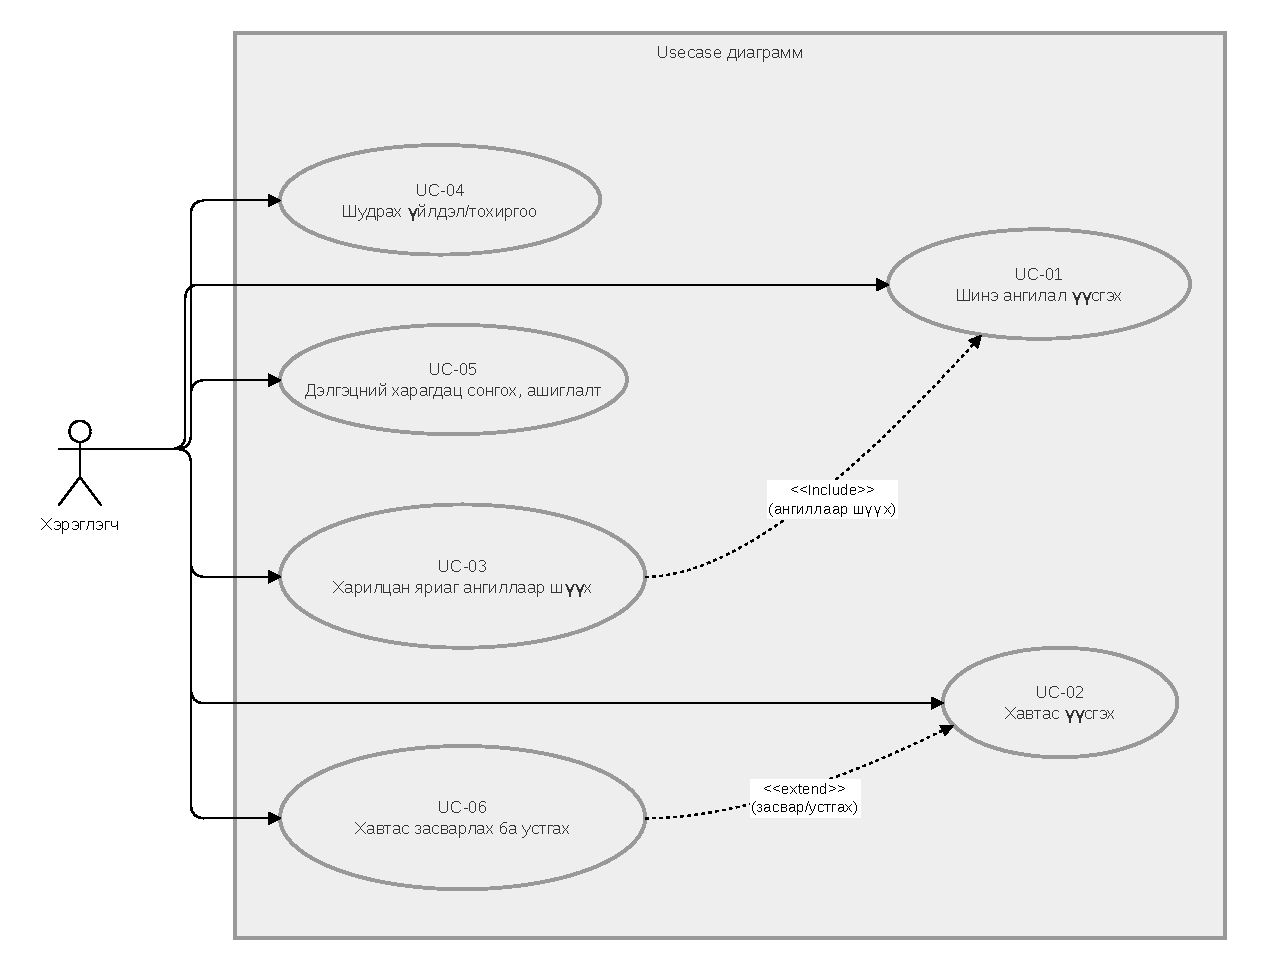
\includegraphics[width=0.85\textwidth]{Diagrams/usecase_diagram.drawio} \caption{Системийн хэрэглээний тохиолдлын диаграмм} \label{fig:usecase_diag} \end{figure}
    Дээрх диаграммд тусгагдсан үндсэн үйлдлүүдийн ажлын урсгал болон нөхцөлүүдийг дараах хүснэгтүүдээр дэлгэрэнгүй тайлбарлав.

% Хэрэглээний тохиолдол 1: Шошго үүсгэх
\begin{longtable}{|l|p{10.5cm}|}
    \caption{Хэрэглээний тохиолдол 1: Шошго үүсгэх} \label{tab:uc_create_category} \\
    \hline
    \textbf{ID / Нэр} & UC-01 / Шинэ шошго үүсгэх \\ \hline
    \textbf{Товч тайлбар} & Хэрэглэгч зурвас шүүх шинэ дүрэм (шошго) үүсгэж, нэр, өнгө болон шүүлтүүрүүдийг тохируулна. \\ \hline
    \textbf{Үйлдэгч} & Хэрэглэгч \\ \hline
    \textbf{Өмнөх нөхцөл} & Хэрэглэгч ``Шошго удирдах'' дэлгэцийг нээсэн байна. \\ \hline
    \textbf{Ажлын урсгал} &
    1. Хэрэглэгч ``+'' товчийг дарж үүсгэх цонхыг нээнэ. \newline
    2. Шошгоны нэрийг оруулж, жагсаалтаас өнгө сонгоно. \newline
    3. Шүүлтүүрийн төрлийг сонгоно: \newline
    \hspace{0.5cm} 3.1. Энгийн үг оруулах бол ``Энгийн үг нэмэх'' талбарт бичнэ. \newline
    \hspace{0.5cm} 3.2. Тогтмол илэрхийлэл (Regex) ашиглах бол дүрс дээр дарж паттерн оруулна. \newline
    4. Оруулсан өгөгдлийг шалгаж ``OK'' товчийг дарна. \\ \hline
    \textbf{Альтернатив} & Хэрэглэгч ``Cancel'' дарвал өөрчлөлт хадгалагдахгүй. Буруу тогтмол илэрхийллийн паттерн оруулбал систем алдаа заана. \\ \hline
    \textbf{Дараах нөхцөл} & Шинэ шошго баазад хадгалагдаж, зурвасууд шууд ангилагдана. \\ \hline
\end{longtable}

\vspace{1em}

% Хэрэглээний тохиолдол 2: Хавтас үүсгэх
\begin{longtable}{|l|p{10.5cm}|}
    \caption{Хэрэглээний тохиолдол 2: Хадгалсан харагдац (Хавтас) үүсгэх} \label{tab:uc_create_folder} \\
    \hline
    \textbf{ID / Нэр} & UC-02 / Хавтас үүсгэх \\ \hline
    \textbf{Товч тайлбар} & Хэрэглэгч өөрийн хэрэгцээнд тохирсон зурвасын харагдац (Хавтас) үүсгэж, доод навигацийн цэсэнд нэмнэ. \\ \hline
    \textbf{Үйлдэгч} & Хэрэглэгч \\ \hline
    \textbf{Ажлын урсгал} &
    1. Баруун дээд цэснээс ``Хавтас'' -> ``Харагдац үүсгэх'' сонгоно. \newline
    2. Хавтасны нэрийг бичиж, харагдах байрлал (index) болон өнгийг тодорхойлно. \newline
    3. ``OK'' товчийг дарж баталгаажуулна. \\ \hline
    \textbf{Дараах нөхцөл} & Шинэ хавтас доод навигацийн цэсэнд нэмэгдэж, хэрэглэгч тухайн хавтас руу автоматаар шилжинэ. \\ \hline
\end{longtable}

\vspace{1em}

% Хэрэглээний тохиолдол 3: Шошгоор шүүх
\begin{longtable}{|l|p{10.5cm}|}
    \caption{Хэрэглээний тохиолдол 3: Шошгоор шүүх} \label{tab:uc_filter_category} \\
    \hline
    \textbf{ID / Нэр} & UC-03 / Харилцан яриаг шошгоор шүүх \\ \hline
    \textbf{Товч тайлбар} & Хэрэглэгч үүсгэсэн хавтас доторх харилцан яриануудыг нэг болон хэд хэдэн шошгоор (Tag) шүүж харна. \\ \hline
    \textbf{Ажлын урсгал} &
    1. Хайх талбарын хажууд байрлах шүүлтүүрийн товчийг дарна. \newline
    2. Гарч ирэх жагсаалтаас нэг болон түүнээс дээш шошгыг сонгоно. \newline
    3. ``OK'' товчийг дарахад систем сонгосон шошгонд таарсан зурвасуудыг харуулна. \\ \hline
    \textbf{Дараах нөхцөл} & Жагсаалт шинэчлэгдэж, шүүлтийн төлөв хадгалагдана. \\ \hline
\end{longtable}

\vspace{1em}

% Хэрэглээний тохиолдол 4: Шудрах үйлдэл
\begin{longtable}{|l|p{10.5cm}|}
    \caption{Хэрэглээний тохиолдол 4: Шудрах үйлдлийн тохиргоо} \label{tab:uc_swipe_actions} \\
    \hline
    \textbf{ID / Нэр} & UC-04 / Шудрах үйлдлийн тохиргоо \\ \hline
    \textbf{Товч тайлбар} & Харилцан ярианы жагсаалтад зүүн эсвэл баруун тийш шудрахад хийгдэх үйлдлийг хэрэглэгч өөрөө сонгоно. \\ \hline
    \textbf{Ажлын урсгал} &
    1. Програмын ерөнхий тохиргооноос ``Шудрах үйлдэл'' хэсгийг нээнэ. \newline
    2. ``Эхнээс нь шудрах'' эсвэл ``Төгсгөлөөс нь шудрах'' сонголтыг дарна. \newline
    3. Боломжит үйлдлүүдээс (Устгах, Архивлах, Уншсан болгох г.м) нэгийг сонгоно. \\ \hline
    \textbf{Дараах нөхцөл} & Сонгосон үйлдэл тэр даруй хадгалагдаж, жагсаалт дээр ажиллаж эхэлнэ. \\ \hline
\end{longtable}

\vspace{1em}

% Хэрэглээний тохиолдол 5: Дэлгэцийн горим
\begin{longtable}{|l|p{10.5cm}|}
    \caption{Хэрэглээний тохиолдол 5: Дэлгэцийн харагдацын горим} \label{tab:uc_screen_view} \\
    \hline
    \textbf{ID / Нэр} & UC-05 / Screen View Mode сонгох \\ \hline
    \textbf{Товч тайлбар} & Нугалдаг төхөөрөмж эсвэл таблет дээр жагсаалт болон дэлгэрэнгүй хэсгийг хэрхэн харуулахыг тохируулна. \\ \hline
    \textbf{Ажлын урсгал} &
    1. Тохиргоо цэсний ``View mode'' хэсэгт орно. \newline
    2. ``Auto'', ``Single'', эсвэл ``Separated'' горимуудаас нэгийг сонгоно. \newline
    3. ``Auto'' горимд систем дэлгэцийн төлөвийг (Дэлгэц хаалттай/нээлттэй) мэдэрч автоматаар шилжинэ. \\ \hline
    \textbf{Дараах нөхцөл} & Програмын үндсэн дэлгэцийн бүтэц (layout) сонгосон горимын дагуу шинэчлэгдэнэ. \\ \hline
\end{longtable}

\vspace{1em}

% Хэрэглээний тохиолдол 6: Хавтас засварлах
\begin{longtable}{|l|p{10.5cm}|}
    \caption{Хэрэглээний тохиолдол 6: Хавтас засварлах ба устгах} \label{tab:uc_edit_folder} \\
    \hline
    \textbf{ID / Нэр} & UC-06 / Хавтас засах эсвэл устгах \\ \hline
    \textbf{Товч тайлбар} & Өмнө үүсгэсэн хавтасны мэдээллийг шинэчлэх эсвэл системээс бүрмөсөн устгана. \\ \hline
    \textbf{Ажлын урсгал} &
    1. Доод навигацийн цэс дээрх хавтасны дүрс дээр удаан дарна. \newline
    2. Мэдээллийг (нэр, өнгө, байрлал) засаад ``OK'' дарах эсвэл ``Delete'' товчийг сонгоно. \newline
    3. Устгах үйлдэл дээр систем дахин баталгаажуулалт асууна. \\ \hline
    \textbf{Дараах нөхцөл} & Өөрчлөлт хадгалагдах эсвэл хавтас навигацийн цэснээс алга болж хэрэглэгч үндсэн харагдац руу шилжинэ. \\ \hline
\end{longtable}

    \paragraph{Төслийн өргөтгөлүүдийн байршил:}
    Дээрх суурь бүтцэд хийсэн өргөтгөлүүд дараах сангуудад нэмэгдсэн:
    \begin{itemize}
        \item \textbf{Regex Filtering логик} – \texttt{messaging/} ба \texttt{extensions/} сангуудад нэмэгдсэн (жишээ нь \texttt{withAutoCategory()}, \texttt{isMessageMatchingCategory()}).
        \item \textbf{Foldable device support} – \texttt{activities/} (\texttt{MainActivity} two-pane логик) болон \texttt{helpers/} (\texttt{FoldableHelper}) хэсэгт хийгдсэн.
        \item \textbf{SavedViews (Folder) систем} – \texttt{models/} (\texttt{SavedView}, \texttt{SavedViewConfig}), \texttt{helpers/} (\texttt{SavedViewsStore}), \texttt{databases/} (Config өргөтгөл) зэрэгт шинээр нэмэгдсэн.
        \item \textbf{Category ба Regex дүрмийн UI} – \texttt{activities/}, \texttt{dialogs/}, \texttt{ui/} (Compose KeywordManager) сангуудад хийгдсэн.
    \end{itemize}
Хөгжүүлэлтийн явцад Git-ийн Feature Branch'' стратегийг \cite{vincent_git} ашиглаж, долоо хоног бүр явцын түүхийг баталгаажуулсан.
 % Үр дүн ба үнэлгээ
    \chapter{Ерөнхий дүгнэлт}

\section{Хийгдсэн ажлын нэгтгэл}
Энэхүү төслийн хүрээнд нээлттэй эхийн Fossify Messages
аппликейшнд суурилан дараах үндсэн бүрэлдэхүүн хэсгүүдийг
амжилттай хөгжүүлж, хэрэгжүүллээ:

\begin{itemize}
    \item \textbf{Тогтмол илэрхийллийн шүүлтүүр}:
    Хэрэглэгчийн тодорхойлсон Regex болон түлхүүр үгэнд
    суурилсан автомат ангиллын алгоритм хэрэгжүүлсэн.

    \item \textbf{Хадгалсан харагдацын систем}:
    Хэрэглэгч өөрийн хэрэгцээнд тааруулсан хавтас
    үүсгэж, зурвасаа ангилан харах боломжийг бүрдүүлсэн.

    \item \textbf{Нугалдаг төхөөрөмжийн дэмжлэг}:
    Samsung Galaxy Z Fold3 дээр хоёр баганат харагдацыг
    гацалтгүйгээр ажиллуулсан.

    \item \textbf{Шудрах үйлдлийн тохиргоо}:
    Хэрэглэгч архивлах, устгах, уншсан тэмдэглэх зэрэг
    үйлдлийг шудрах хөдөлгөөнд оноох боломжтой болсон.

    \item \textbf{Хугацааны бүлэглэлт}:
    Inbox дахь харилцан яриануудыг өнөөдөр, өчигдөр,
    энэ сар гэсэн бүлгүүдэд автоматаар ангилдаг болсон.
\end{itemize}

\section{Зорилгын биелэлт}
Chapter 1-д SMART зарчмаар тавьсан зорилгуудын биелэлтийг
дараах байдлаар нэгтгэв:

\begin{table}[H]
    \centering
    \caption{SMART зорилгын биелэлтийн нэгтгэл}
    \label{table:smart_result}
    \begin{tabular}{|l|p{5cm}|c|}
        \hline
        \textbf{Зорилго} & \textbf{Үр дүн} & \textbf{Биелэлт} \\
        \hline
        Specific & Тогтмол илэрхийлэл болон түлхүүр үгэнд суурилсан
        автомат ангилал хэрэгжсэн & \checkmark \\
        \hline
        Measurable & 31 тест 100\% Pass,
        гол логикийн coverage ~85\% & \checkmark \\
        \hline
        Achievable & Нугалдаг төхөөрөмж дээр
        тасралтгүй 2 баганат харагдац & \checkmark \\
        \hline
        Relevant & Нээлттэй эхийн орчинд
        хэрэгжүүлсэн & \checkmark \\
        \hline
        Time-bound & Хамгаалалтын өмнө
        бүрэн ажиллагаатай & \checkmark \\
        \hline
    \end{tabular}
\end{table}

\section{Туршилтын үр дүнгийн нэгтгэл}
Системийн найдвартай ажиллагааг баталгаажуулахын тулд
нэгж туршилт, нэгтгэл туршилт болон ачааллын туршилт
гүйцэтгэсэн үр дүнг дараах байдлаар нэгтгэв:

\begin{itemize}
    \item \textbf{Нэгж туршилт}: 31 тест, 100\% Pass
    \item \textbf{Цөм логикийн кодын хамралт}: ~85\%
    \item \textbf{Ачааллын туршилт}: 40,000 харилцан яриа,
    дунджаар 15мс-ээс бага хариу хугацаа
    \item \textbf{Бодит төхөөрөмж}: Samsung Galaxy Note20 Ultra
    болон Z Fold3 дээр бүх үндсэн функцүүд амжилттай ажилласан
\end{itemize}

\section{Хязгаарлалт}
Төслийн хүрээнд дараах зүйлсийг хэрэгжүүлэх боломжгүй
байсан тул цаашдын ажил болгон үлдээв:

\begin{itemize}
    \item CI/CD pipeline-г Fossify-ийн нарийн
    build dependency-аас шалтгаалан бүрэн автоматжуулж
    чадаагүй
    \item Fossify Messages repository-д өөрийн хөгжүүлсэн функцуудыг нэгтгээгүй.
\end{itemize}

\section{Цаашдын хөгжүүлэлт}
Энэхүү төсөл нь цаашид илүү өргөжүүлэн хөгжүүлж,
хэрэглэгчдийн өдөр тутмын амьдралыг илүү хялбаршуулах
бүрэн боломжтой юм. Тэргүүлэх чиглэлүүд:

\begin{itemize}
    \item \textbf{Шүүх механизмын сайжруулалт}:
    Ангилалах дүрэмд нэмэлт нөхцөлүүдийг (жишээ нь: Харилцагчын бүлэг, ангилагдахгүй нөхцөл, цаг хугацаа гэх мэт) нэмж, илүү нарийн ангилал хийх боломжийг бий болгох
    \item \textbf{CI/CD бүрэн нэвтрүүлэлт}:
    GitHub Actions pipeline-г тогтворжуулж,
    автомат тест болон APK build-ийг хэрэгжүүлэх
    \item \textbf{Агуулгад суурилсан функцууд}:
    Ангиллын дагууд мэдэгдэл тохируулах боломжийг нэмэх, агуулгыг танаж багасгах
    \item \textbf{Fossify Messages-т нэгтгэх}:
    Нийтэд нээлттэй репозиторт өөрийн хөгжүүлсэн кодыг нэгтгэж,
    нээлттэй эх бүхий программ хангамж хөгжүүлэгчдийн нийгэмлэгийн хамтын ажиллагаанд нэмэр болох
\end{itemize}

Өдөр тутмын амьдралд бидэнд бэлэн өгөгддөг зүйлсийг
өөрийн хэрэгцээ шаардлагын дагуу өөрчилж, сайжруулснаар
ямар их эерэг өөрчлөлтийг авчирч болдгийг энэхүү ажил харууллаа.
 % Дүгнэлт ба цаашдын ажил
% Ном зүй (Ашигласан материал)
    \cleardoublepage
    \defformat
    \nocite{*}
    \addchap{Ном зүй}
    \printbibliography[heading=none]

% Хавсралт
    \appendix
    \chapter{Эх кодын холбоосууд}
\label{AppendixA}

Энэхүү дипломын ажлын хүрээнд хийгдсэн өөрчлөлтүүд болон үндсэн төслийн эх кодуудтай дараах хаягуудаар танилцах боломжтой:

\begin{itemize}
    \item \textbf{Төслийн үндсэн github холбоос} \\
    \url{https://github.com/Timekilla-tech/Messages}

    \item \textbf{Fossify Messages (Үндсэн төсөл):} \\
    \url{https://github.com/FossifyOrg/Messages}
\end{itemize}

\vspace{2em}


\end{document}
